%\documentclass[10pt, twocolumn]{article}
%\documentclass[11pt]{article}
%\documentclass[twocolumn,showpacs,preprintnumbers,amsmath,amssymb,prl, superscriptaddress]{revtex4}
\documentclass[twocolumn,preprintnumbers,amsmath,amssymb,prd, superscriptaddress]{revtex4}
% \documentclass[preprintnumbers,amsmath,amssymb,prd,superscriptaddress]{revtex4}
%\documentclass[10pt, preprint,showpacs,preprintnumbers,amsmath,amssymb, superscriptaddress]{revtex4}
%\documentclass[11pt, prd,preprintnumbers,amsmath,amssymb, superscriptaddress]{revtex4}
%\documentclass[11pt, prd,preprintnumbers, amsmath,amssymb, superscriptaddress, nofootinbib, hyperref]{revtex4}


\usepackage{latexsym}
\usepackage{amssymb}
\usepackage{epsfig,amsmath,graphics}
\usepackage{epstopdf}
\usepackage{verbatim}
\usepackage{wasysym}
\usepackage{hyperref}
\usepackage{feynmp-auto} % feynman diagrams
%\usepackage{subfig}
\usepackage[utf8]{inputenc}
\usepackage{xpatch}
\usepackage{xcolor}
\usepackage{mathtools}
\hypersetup{
    colorlinks,
    linkcolor={red!80!black},
    citecolor={green!60!black},
    urlcolor={blue!60!black}
}
\usepackage{appendix}

\newcommand{\Ez}{\mathcal{E}_0}
\newcommand{\Eboom}{\mathcal{E}_\text{boom}}
\newcommand{\OO}{\mathcal{O}}
\newcommand{\LL}{\mathcal{L}}
\newcommand{\HH}{\mathcal{H}}
\newcommand{\TeV}{\text{TeV}}
\newcommand{\GeV}{\text{GeV}}
\newcommand{\MeV}{\text{MeV}}
\newcommand{\keV}{\text{keV}}
\newcommand{\rad}{\text{rad}}
\newcommand{\cm}{\text{cm}}
\newcommand{\angstrom}{\buildrel _{\circ} \over {\mathrm{A}}}
\newcommand{\pslash}{p\hspace{-0.070in}/\,}
\newcommand{\Mpl}{M_{\text{pl}}}
\newcommand{\ket}[1]{\ensuremath{\left|#1\right>}}
\newcommand{\bra}[1]{\ensuremath{\left<#1\right|}}
\newcommand{\braket}[2]{\ensuremath{\left<#1|#2\right>}}
%Large Parentheses
\def\r{\right)}
\def\l{\left(}

\begin{document}

%\preprint{APS/123-QED}


\title{White Dwarfs as Dark Matter Detectors}

\author{Peter W. Graham}
\affiliation{Stanford Institute for Theoretical Physics, Department of Physics,
Stanford University, Stanford, CA, 94305}

\author{Ryan Janish}
\affiliation{Berkeley Center for Theoretical Physics, Department of Physics,
University of California, Berkeley, CA 94720, USA}

\author{Vijay Narayan}
\affiliation{Berkeley Center for Theoretical Physics, Department of Physics,
University of California, Berkeley, CA 94720, USA}

\author{Surjeet Rajendran}
\affiliation{Berkeley Center for Theoretical Physics, Department of Physics,
University of California, Berkeley, CA 94720, USA}

\author{Paul Riggins}
\affiliation{Berkeley Center for Theoretical Physics, Department of Physics,
University of California, Berkeley, CA 94720, USA}

\begin{abstract}

If dark matter (DM) were capable of sufficiently heating a localized region of a white dwarf, it would trigger runaway fusion and ignite a type 1a supernovae. 
This was originally proposed in \cite{Graham:2015apa} and used to constrain primordial black holes which transit a white dwarf and cause heating through dynamical friction. 
In this paper, we extend the reach of white dwarf DM detectors to candidates with non-gravitational interactions that cause heating through the release of standard model particles. 
We consider a general class of models in which DM-DM annihilations, DM decays, or DM scatters produce particles that subsequently deposit their energy inside the star.  
The existence of certain, long-lived white dwarfs and the measured supernovae rate provide robust methods for constraining such models. 
As a concrete example, we are able to rule out supersymmetric Q-ball DM in a vast region of parameter space fundamentally inaccessible to terrestrial-based experiments.
It is interesting that the DM encounters with white dwarfs discussed in this work provide an alternative mechanism of triggering supernovae from sub-Chandrasekhar Mass progenitors. 


\end{abstract}
\maketitle
\tableofcontents
\clearpage

\section{Introduction}
\label{sec:Introduction}

Identifying the nature of dark matter (DM) remains one of the clearest paths beyond the Standard Model (SM).
Therefore, it is fruitful to study the observable signatures of any yet-allowed candidate.
Many terrestrial direct section experiments have been designed to search for DM, yet these lack sensitivity to ultra-heavy DM due to its diminished number density and local flux.
Even for a strongly-interacting candidate, if the DM mass is above $\sim 10^{22} ~\GeV$ a large detector of size $\sim (100 ~\text{m})^2$ will register fewer than a one event per year.
While these masses are large compared to those of fundamental particles, it is reasonable to suppose that DM may exist as composite states just as the SM produces complex structures with mass much larger than fundamental scales (e.g., you, dear reader).
Currently there is a wide range of unexplored parameter space for ultra-heavy DM candidates less than $\sim 10^{48} ~\GeV$, at which point the DM will have observable gravitational microlensing effects. 
For such ultra-heavy DM, indirect signatures in astrophysical systems are a natural way forward.
One possibility originally proposed by \cite{Graham:2015apa} is that DM can trigger runaway fusion and ignite type 1a supernovae (SN) in sub-Chandrasekhar white dwarf (WD) stars.

Runaway fusion requires both a heating event and the lack of significant cooling which might quench the process.
The WD medium is particularly suited to this, since it is dominated by degeneracy pressure and undergoes minimal thermal expansion, which is the mechanism that regulates fusion in main sequence stars.
Thermal diffusion is the dominant cooling process, which can be thwarted by heating a large enough region.
The localized heating necessary to trigger runaway fusion was computed in \cite{Woosley} and recently used in \cite{Graham:2015apa} to place bounds on primordial black hole DM.
In addition, \cite{Graham:2015apa} identifies other heating mechanisms which may be similarly constrained, including the production of high energy SM particles within the WD.
Here we focus on this scenario.
It is important to note these constraints are complimentary to terrestrial ones---it is more massive DM that is likely to trigger SN, but also more massive DM that has low terrestrial flux.
The WD detector excels in this regime due to its large surface area, long lifetime, and galactic abundance.

An essential ingredient in this analysis is understanding how SM particles deposit energy in a WD medium
We find that most high energy particles tend to thermalize efficiently with ions in the WD, nearly independent of the particle species or energy.
Particle production is thus an effective means of inducing SN, and the WD may be thought of as a detector with hadronic and electromagnetic ``calorimeter'' components.
This is used to constrain DM models with a variety of SM production modes: DM-DM collisions or DM decays, transits with a DM-SM scattering interaction, and DM capture scenarios.
The bounds are due to either observing specific, long-lived WDs or by comparing the measured type Ia SN rate with the much larger rate expected due to DM events.
As a concrete example, Q-balls found in supersymmetric extensions of the SM provide an ultra-heavy DM candidate of this type.
We constrain a large region of Q-ball DM parameter space that is fundamentally inaccessible to terrestrial experiments.

We begin in Section~\ref{sec:Review} by reviewing the mechanism of runaway fusion in a WD.
The bulk of the work is done in Section~\ref{sec:SMHeating}, where we study the heating properties of SM particles and determine when the production of such particles results in a SN.
Detailed calculations of SM energy loss in the WD medium are provided in Appendix \ref{sec:Appendix}.
In Section~\ref{sec:DMexplode} we parameterize the modes of DM-WD interaction that may produce SM particles, and in Section~\ref{sec:Constraints} we derive kinematics constraints on these interactions.
We examine the specific case of Q-ball DM in Section~\ref{sec:QBalls}, and conclude in Section~\ref{sec:Discussion}.

\section{White Dwarf Runaway Fusion}
\label{sec:Review}

We review here the conditions in which a local energy deposit in a carbon-oxygen WD results in runaway fusion.
Any energy deposit will eventually heat carbon ions within some localized region.
Parameterize this region by a linear size $L_0$ and peak temperature $T_0$.
These scales evolve in time, but it will be useful to describe a given heating event by their initial values.

The fate of a heated region is either a nonviolent diffusion of the excess energy across the star, or a runaway fusion chain-reaction that destroys the star.
The precise outcome depends on both $L_0$ and $T_0$.
There is a critical fusion temperature $T_f$, set by the energy required for ions to overcome their mutual Coulomb barrier, above which fusion occurs.
For carbon-carbon fusion, $T_f \sim \MeV$ \cite{Gasques:2005ar}.
Any event with $T_0 > T_f$ will initially support fusion, however this condition is not sufficient for triggering runaway as cooling processes may quickly lower the temperature below $T_f$.
This cooling will not occur if the cooling timescale is larger than the timescale at which fusion releases energy.

Cooling in a WD is dominated by thermal diffusion, the timescale for which increases with the size of heated region.
However, the timescale for heating due to fusion is independent of region size.
Thus, for a given temperature $T\gtrsim T_f$, there is always a critical size above which the heated region does not cool and initiates nuclear runaway.
For a region at the fusion threshold $T \sim T_f$, this critical size is what we will call the \emph{trigger size} $\lambda_T$.
The value of $\lambda_T$ is highly dependent on density, and in a WD is set by the thermal diffusivity of either photons or degenerate electrons.
It has been calculated numerically in \cite{Woosley} and scaled for varying WD masses in \cite{Graham:2015apa}.
This is plotted in \textcolor{blue}{figure (same one with MeV thermalization lengths)}.
As in \cite{Graham:2015apa}, we restrict our attention to carbon-oxygen WDs in the upper mass range $\sim 0.85 - 1.4 ~M_{\odot}$ - we will see that only these give meaningful constraints.
This mass range correspond to a central number density of ions $n_\text{ion} \sim 10^{30} - 10^{32} ~\cm^{-3}$ and a trigger size of $\lambda_T \sim 10^{-3} - 10^{-5} ~\text{cm}$.
If a heated region is smaller than $\lambda_T$, its thermal evolution is initially dominated by diffusion.
However, at a later time this may still result in runaway fusion if the temperature remains above $T_f$ by the time the region has diffused out to the trigger size.
This yields the \emph{boom condition} for a heating event ($L_0$, $T_0$):
\begin{align}
    \label{eq:Tboom}
    % T_0 \gtrsim T_f \cdot \text{max}\left\{1, \frac{\lambda_T}{L_0}\right\}^3
    T_0 \gtrsim \begin{cases}
      T_f & L_0 \gtrsim \lambda_T \\
      T_f \left( \frac{\lambda_T}{L_0} \right)^3 & L_0 \lesssim \lambda_T
    \end{cases}
\end{align}

It will be more useful for our purposes to phrase this condition in terms of the total energy $\Ez$ deposited during a heating event.
The relation between $\Ez$ and $T_0$ will depend on which WD constituents (ions, degenerate electrons, and photons) are heated.
These species are coupled, however, by electromagnetic interactions.
The lengths over which they mutually thermalize when heated to $\sim T_f$ are plotted in \textcolor{blue}{figure}, and as these are all smaller than the trigger size we will have all three species in equilibrium during any event capable of runaway:
\begin{equation}
  \frac{\Ez}{V} \gtrsim \int_0^{T_f} dT ~\left(\frac32 n_\text{ion} + \frac{\pi^{4/3}}{3^{1/3}}\, n_e^{2/3} T + \frac{4 \pi^2}{15} T^3 \right)
  % confirm the Fermi gas coefficient
\end{equation}
Note that $n_e$ is the electron density, and this contribution uses the heat capacity of a degenerate gas as the Fermi energy $E_F \gtrsim T_f$ for the densities we consider.
The absolute minimal ignition energy is
\begin{align}
\label{eq:Eboom}
\Eboom &\sim \frac{4 \pi}{3} \lambda_T^3 (n_\text{ion} T_f + n_e^{2/3} T_f^2 + T_f^4) \\
         &\sim  10^{15} - 10^{23} ~\GeV \nonumber,
\end{align}
which varies with $\lambda_T$ over the range of WD densities. % the coefficients are actually ~1.5, 1.6, and 0.7, respectively
This is plotted in Figure \ref{fig:Eboom}.
The boom condition~\eqref{eq:Tboom} can be restated as
\begin{align}
    \label{eq:energy_boom_condition}
    \Ez \gtrsim
    \Eboom \cdot \text{max}\left\{1, \frac{L_0}{\lambda_T}\right\}^3.
\end{align}
The energy needed for ignition is thus minimized for heating lengths $L_0$ less than the trigger size, where it is also independent of the precise value of $L_0$.
For broader deposits, the required energy is parametrically larger than $\Eboom$ by a volume ratio $(L_0/\lambda_T)^3$.
Understanding the heating lengths $L_0$ resulting from the production of SM particles is therefore critical to determining whether or not these processes are capable of destroying a WD.


\begin{figure}
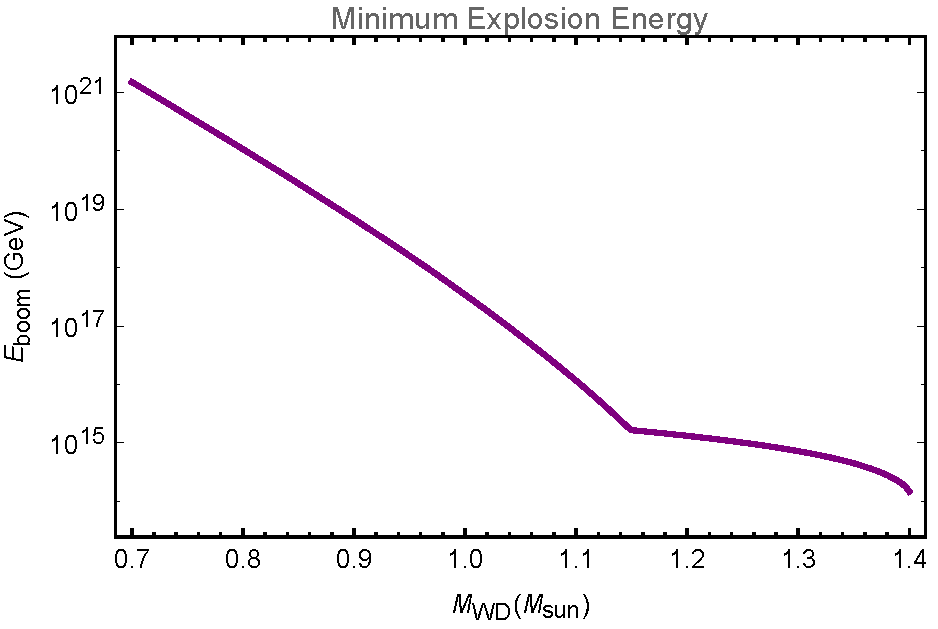
\includegraphics[scale=.45]{Eboom.pdf}
\caption{Minimum energy $\Eboom$ (see equation \eqref{eq:Eboom}) required to trigger SN as a function of WD mass, based on numerical results for $\lambda_T$ \cite{Woosley} and the WD mass-density relation \cite{cococubed}}
\label{fig:Eboom}
\end{figure}

\section{Non-Gravitational Heating of White Dwarfs}
\label{sec:SMHeating}

Having reviewed the requirements for runaway fusion in a WD, we turn to the question of triggering these events with DM.
This amounts to determining the heating length $L_0$ and energy deposit $\Ez$ due to a given DM encounter with a WD---if condition \eqref{eq:energy_boom_condition} is satisfied, then the encounter is explosive.
Of course, the parameters $L_0$ and $\Ez$ necessarily depend on the nature of the DM and must be explicitly calculated for a given DM model.
In particular, any DM candidate which couples to the SM will generically be able to release SM secondaries which then thermalize with stellar constituents.
For these types of processes, the unknown DM physics serves only to determine the initial distribution in space, energy, and species of the SM particles produced in the star, while the actual heating proceeds entirely though known SM interactions.
It is therefore necessary to understand how energy is transferred from SM particles to the stellar medium in order to assess the explosiveness of these encounters.

The remainder of this Section is dedicated to computing the heating properties of SM species in a manner that is independent of the DM encounter.
We summarize here the dominant source of energy loss for each species while a more detailed treatment of particle interactions in a WD is reserved for Appendix \ref{sec:Appendix}. In particular, we consider light hadrons, electrons, photons, and neutrinos released in the WD.

Consider a schematic energy deposition in which $N$ particles of a single SM species and uniform energy $\epsilon$ are released isotropically in the stellar interior.
As we are primarily concerned with triggering runaway fusion, it is sufficient to take $\epsilon \gg T_f \sim \text{MeV}$.
In addition, either a few $N \sim 1$ ultra-high energy particles or a large number $N \gg 1$ of lower energy particles can be released.
These scenarios may have vastly different heating lengths, and we distinguish between the two when applicable.
The heating length $L_0$ of any such deposition is ultimately determined by the distances individual particles travel in a WD before giving up $\OO(1)$ of their energy.
This range can determined from the stopping powers $(dE/dx)$ for different interactions, which are explicitly calculated in Appendix \ref{sec:Appendix}.
It is important to note that if a process predominantly transfers energy to electrons or additional secondaries, the relevant length scale $L_0$ will be the larger distance over which \emph{ions} are eventually heated.

\subsection{Heating Properties: Hadrons}

For high-energy incident hadrons, the energy loss is dominated by inelastic nuclear collisions in which the incoming hadron violently interacts with a target nucleus to produce an $\OO(1)$ number of secondary hadrons.
This results in a roughly collinear hadronic shower that terminates when shower constituents reach a critical energy $E_\text{crit}$.
These final-state hadrons will consist of roughly equal fractions of pions, protons, and neutrons.
For neutrons, $E_\text{crit}$ is of order the nuclear binding energy $\sim 10 ~\text{MeV}$ although for charged hadrons, it is either $\sim 10 ~\MeV$ or the energy when Coulomb collisions with electrons becomes dominant.
The precise value of $E_\text{crit}$ is a nontrivial function of the WD density.
The shower length is determined by the typical mean free path $l_\text{inel}$ and cross-section $\sigma_\text{inel} \approx 100 ~\text{mb}$ for inelastic collisions:
\begin{align}
\label{eq:hadlength}
  X_\text{had} \sim l_\text{inel} \log\l\frac{\epsilon}{E_\text{crit}}\r
  \approx 10^{-6} ~\text{cm} \l\frac{10^{32}~\text{cm}^{-3}}{n_\text{ion}}\r.
\end{align}
As a result, a high-energy nucleon or pion ultimately transfers its energy to many low-energy hadrons, displaced a distance $X_\text{had}$ from its starting point.
Note that neutral pions decay to photons with a mean lifetime $\sim 10^{-16} ~\text{s}$, so that a $10 - 100 ~\text{MeV}$ neutral pion has a decay length of order $\sim 10^{-6} ~\text{cm}$.
Hence, there will be negligible electromagnetic contributions from $\pi^0$ decays during the progression of a hadronic shower.
For simplicity we focus on the hadronic component, which will carry a significant fraction of the shower energy.

At energies less than $\sim 10 ~\MeV$, protons and neutrons are predominantly stopped by elastic nuclear scatters, characterized by a mean free path $l_\text{el}$ and cross-section $\sigma_\text{el} \approx 1 ~\text{b}$.
On the other hand, charged pions will primarily transfer their energy to electrons in the stellar medium via Coulomb collisions.
Nevertheless, since each final-state nucleon and pion species carries $\OO(1)$ of the initial energy, a reasonable estimate of the heating length is obtained by considering only the final energy deposition from protons and neutrons.
We find that $\sim 10$ random-walk collisions are needed to slow $\sim 10 ~\MeV$ nucleons to $\sim \MeV$ energies, resulting in an elastic scattering distance of order
\begin{equation}
 \lambda_\text{el} \sim \sqrt{10} \times l_\text{el} \approx 10^{-7} ~\text{cm} \l\frac{10^{32}~\text{cm}^{-3}}{n_\text{ion}}\r
\end{equation}
If a single high-energy hadron $N \sim 1$ is released in the WD, the resulting ion temperature profile will be displaced from the origin by the hadronic shower length $X_\text{had}$ with characteristic size $L_0 \sim \lambda_\text{el}$.
If instead many hadrons $N \gg 1$ are initially released and thermalize collectively, the heating length will be of order $L_0 \sim X_\text{had} + \lambda_\text{el} \approx X_\text{had}$.
In either case, the heating length is parametrically smaller than the trigger size $\lambda_T$ and so the release of high-energy hadrons is an efficient heating mechanism for WDs.

\subsection{Heating Properties: Electrons and Photons}

We now consider the heating properties of electrons and photons together as their interactions are highly coupled.
In this case, the dependence on WD density is not as straightforward due to the LPM effect, which suppresses radiative processes at high densities.
We explicitly calculate the heating of a WD $n_\text{ion} \sim 10^{32} ~\cm^3$, although it is straightforward to generalize these results to lower densities - the only difference will be the turning points that characterize the dominance of one interaction over another.


At low energies, $\epsilon \lesssim 10~\GeV$, both electrons and photons primarily lose energy via elastic scattering off WD electrons.
Thus the first stage of heating will be to establish a region of heated electron gas.
Once the electrons equilibrate, they will begin to further lose energy via the previously sub-dominant bremsstrahlung process - this increases the photon number density, which transfers energy back into electrons by Compton scatters, and will eventually lead to the thermalization of the electrons and photon.
The establishment of this heated electron-photon gas will occur significantly before any energy is transfered to ions, as evidenced by the hierarchy between the electron-ion and photon-ion stopping powers and the election-photon stopping powers in Figure \ref{fig:SOMETHING}.
If the process originally released $N$ electrons or photons of energy $\epsilon \lesssim 10~\GeV$, then this electron-photon gas has a temperature of
\begin{align}
  T_{e\gamma} \sim \frac{N \epsilon}{Z n_\text{ion} \lambda_{e\gamma}^3}
\end{align}
where $\lambda_{e\gamma}$ is the range of electrons due to bremsstrahlung and we assume that $N$ is sufficiency large so that $T_{e\gamma} \gtrsim 1~\MeV$.

Note that if $T_{e\gamma} \lesssim 10~\MeV$, the only routes to transfer energy to ions are dramatically suppressed.
In that case, ion heating is dispersed over an insignificantly large region.
However, if $T_{e\gamma} \gtrsim 10~\MeV$, then photons in this gas will transfer their energy to ions via photonuclear scatters, which are nonelastic nuclear scatters as discussed in Section \ref{sec:SOMETHING} between a photon and a nucleus, mediated by a virtual quark pair.
As $N$ is large and each photon carries a small fraction of the total deposited energy, the effect here is to launch many hadronic showers from the electron-photon gas which heat ions as discussed.
The total length of these photo-nuclear showers is given by $l_\gamma + X_\text{had}$, where $X_\text{had}$ is the hadronic shower length and $l_\gamma$ the mean free path for a photonuclear collision, which is related to the hadronic mean free path for nonelastic nuclear collisions by $\sim l_\text{h,non}/\alpha$.
The photonuclear piece dominates, and it also dominates the initial scale of the heated electrons and photons $\lambda_{e\gamma}$, so we find that a low-energy cloud of electrons or photons will eventually heat ions over a distance $\sim l_\gamma$.

For slightly larger energies, there is a narrow window $10~\GeV \lesssim \epsilon \lesssim 100~\GeV$ in which both electrons and photons are dominated by radiative processes.
In this regime we thus have an EM shower, which terminated at energies of $\sim 10~\GeV$ into a cloud of electrons and photons, which thermalize as described above.
This is a collinear shower covering about a decade in energy, so its principle effect is to amplify the number of energetic particles by a factor of $10$ and to disperse them over an EM shower length (note that since many particles are necessary involved here, this is a broadening of the heating peak and not a displacement).
If $N$ electrons or photons are released with energy $\epsilon$ and create EM showers, the shower products with thermalize an electron-photon gas of temperature
\begin{align}
  T_{e\gamma} \sim \frac{10 N \epsilon}{Z n_\text{ion} X_\text{EM}^3}
\end{align}
where $X_\text{EM}$ is the length of the EM shower.
At these densities, the shower lengths are extended by the LPM effect and given by
\begin{align}
  X_\text{EM} \sim X_0 \l \frac{\epsilon}{E_\text{LPM}} \r^{1/2},
\end{align}
where $E_\text{LPM} \sim$ \textcolor{blue}{NUMBERS} and $X_\text{EM} \sim$ \textcolor{blue}{NUMBERS}. \textcolor{blue}{citation}
As above, if $T_{e\gamma} \gtrsim 10~\MeV$ this will produce photonuclear hadronic showers and heat the ions over a scale $l_\gamma$.

Finally, at high energies $\epsilon \gtrsim 100~\GeV$ a released photon or electron will deposit energy directly into hadronic showers without first thermalizing a region of electron-photon gas.
Effectively, electrons and photons at this energy behave qualitatively like hadrons, with the quantitative difference in that they require a slightly longer distance to initiate a hadronic shower.
The physics is the same as that discussed in Section \ref{sec:SOMETHING}, though we now must add a photonuclear or electronucler length scale to the shower length $X_\text{had}$.
For $100~\GeV \lesssim \epsilon \lesssim 1~\TeV$, the shower is always photonuclear, as a released electron is more likely to bremsstrahlung than scatter off a nucleus and that bremmed photon is then able to start a photonuclear shower.
For $\epsilon \gtrsim 1~\TeV$, however, released electrons will start hadronic showers directly by radiating a virtual photon which undergoes a photonuclear collision.
This slows the electron over a length scale $\sim 10~l_\gamma/\alpha \sim 10 l_\text{h,non}/\alpha^2 $.

\subsection{Heating Properties: Neutrinos}

Neutrinos interact very weakly, although their nuclear cross-section $\sigma_{\nu A}$ rises with energy.
At an energy of $\sim 10^{11} ~\GeV$, \cite{Formaggio:2013kya} calculates the cross-section to be $\sigma_{\nu A} \sim 10^{-32} ~\cm^2$.
Taking this to be a conservative estimate for nuclear cross-section at even higher energies, we find the mean free path for a neutrino-nuclei scatter is of order $\sim \text{meter}$.
However, if we consider the release of a single ultra-high energy neutrino, than this mean free path is simply a displacement of the eventual thermal profile.
In a nuclear interaction, $20 \%$ of the neutrino energy is transferred to the nucleus while the rest is transferred to produced electrons \cite{Formaggio:2013kya}.
In this case, the energy deposited to the nucleus is sufficient to start a hadronic shower.
Therefore, a ultra-high energy neutrino behaves like a hadron and the neutrino heating length is simply $L_0 \sim X_\text{had}$.

\section{Dark Matter-Induced Ignition}
\label{sec:DMexplode}

We now consider those aspects of DM-induced heating of WDs by SM particle production that depend on the nature of DM and its interactions with the SM.
Of course, the unknown DM physics determines the distribution in momentum, species, and space of particles produced in the star - this must be known in order to determine if the DM-WD encounter is capable of triggering a SN and the rate of such events. 
In this Section, we remain agnostic about the identity of DM and instead consider several illustrative classes of DM-SM interaction which demonstrate simply the sorts of constraints obtained by considering DM-induced ignition.
We describe these interactions below and compute their .
Constraints for these processes are given in Section~\ref{sec:Constraints}.

\subsection{Classifying Dark Matter - White Dwarf Encounters}

DM may be generically expected to interact with the WD medium through the three processes depicted in Figure \ref{fig:feynman}: DM-DM collisions, DM decays, and DM-SM scattering.
Note that for ultra-heavy DM these processes may not be elementary interactions, but possibly more complicated events involving many (potentially dark sector) final states, analogous to the interactions of heavy nuclei.
We classify DM candidates into three types according to the interaction that provides the dominant source of heating, and refer to theses are decay, collision, and transit candidates.
We also make some simplifying assumptions about the spatial extent of these interactions.
We consider only decays and collisions that are point-like, with all SM products produced in a localized region (smaller than the trigger size).
For transits, we consider only soft DM-SM scatters that result in a continuous release of SM energy along the DM trajectory.

We additionally classify candidates according to the evolution of the DM itself inside the star.
There will be some loss of kinetic energy due to DM-SM scatters.
This may be incidental to the eventual heating of the star, e.g.~in the case of heating by DM decays, or it may represent the dominant heating process.
We consider two simple limiting scenarios depending on the magnitude of this energy loss: ``DM wind" and ``DM capture".
In the ``wind" case only a small fraction of the DM kinetic energy is lost and it simply passes through the star, whereas in the ``capture" case the energy loss is sufficient to stop the DM and cause it to accumulate inside the star.
We will consider both wind and capture scenarios for DM that heats by annihilations or decays, as for these models the capture scenario has a significantly enhanced rate of events.
For simplicity, we consider only the wind scenario for transit candidates, though an enhancement of the heating due to capture is certainly possible in some models.

Finally, a realistic interaction will produce SM particles with some distribution in momentum and species that ought to be summed over to asses the resulting heating.
In what follows, however, for simplicity we will assume that each interaction produces particles of a single species $i$ and energy $\epsilon$.
This will demonstrate the typical scale of the resulting constraints on DM parameters.

\begin{figure}
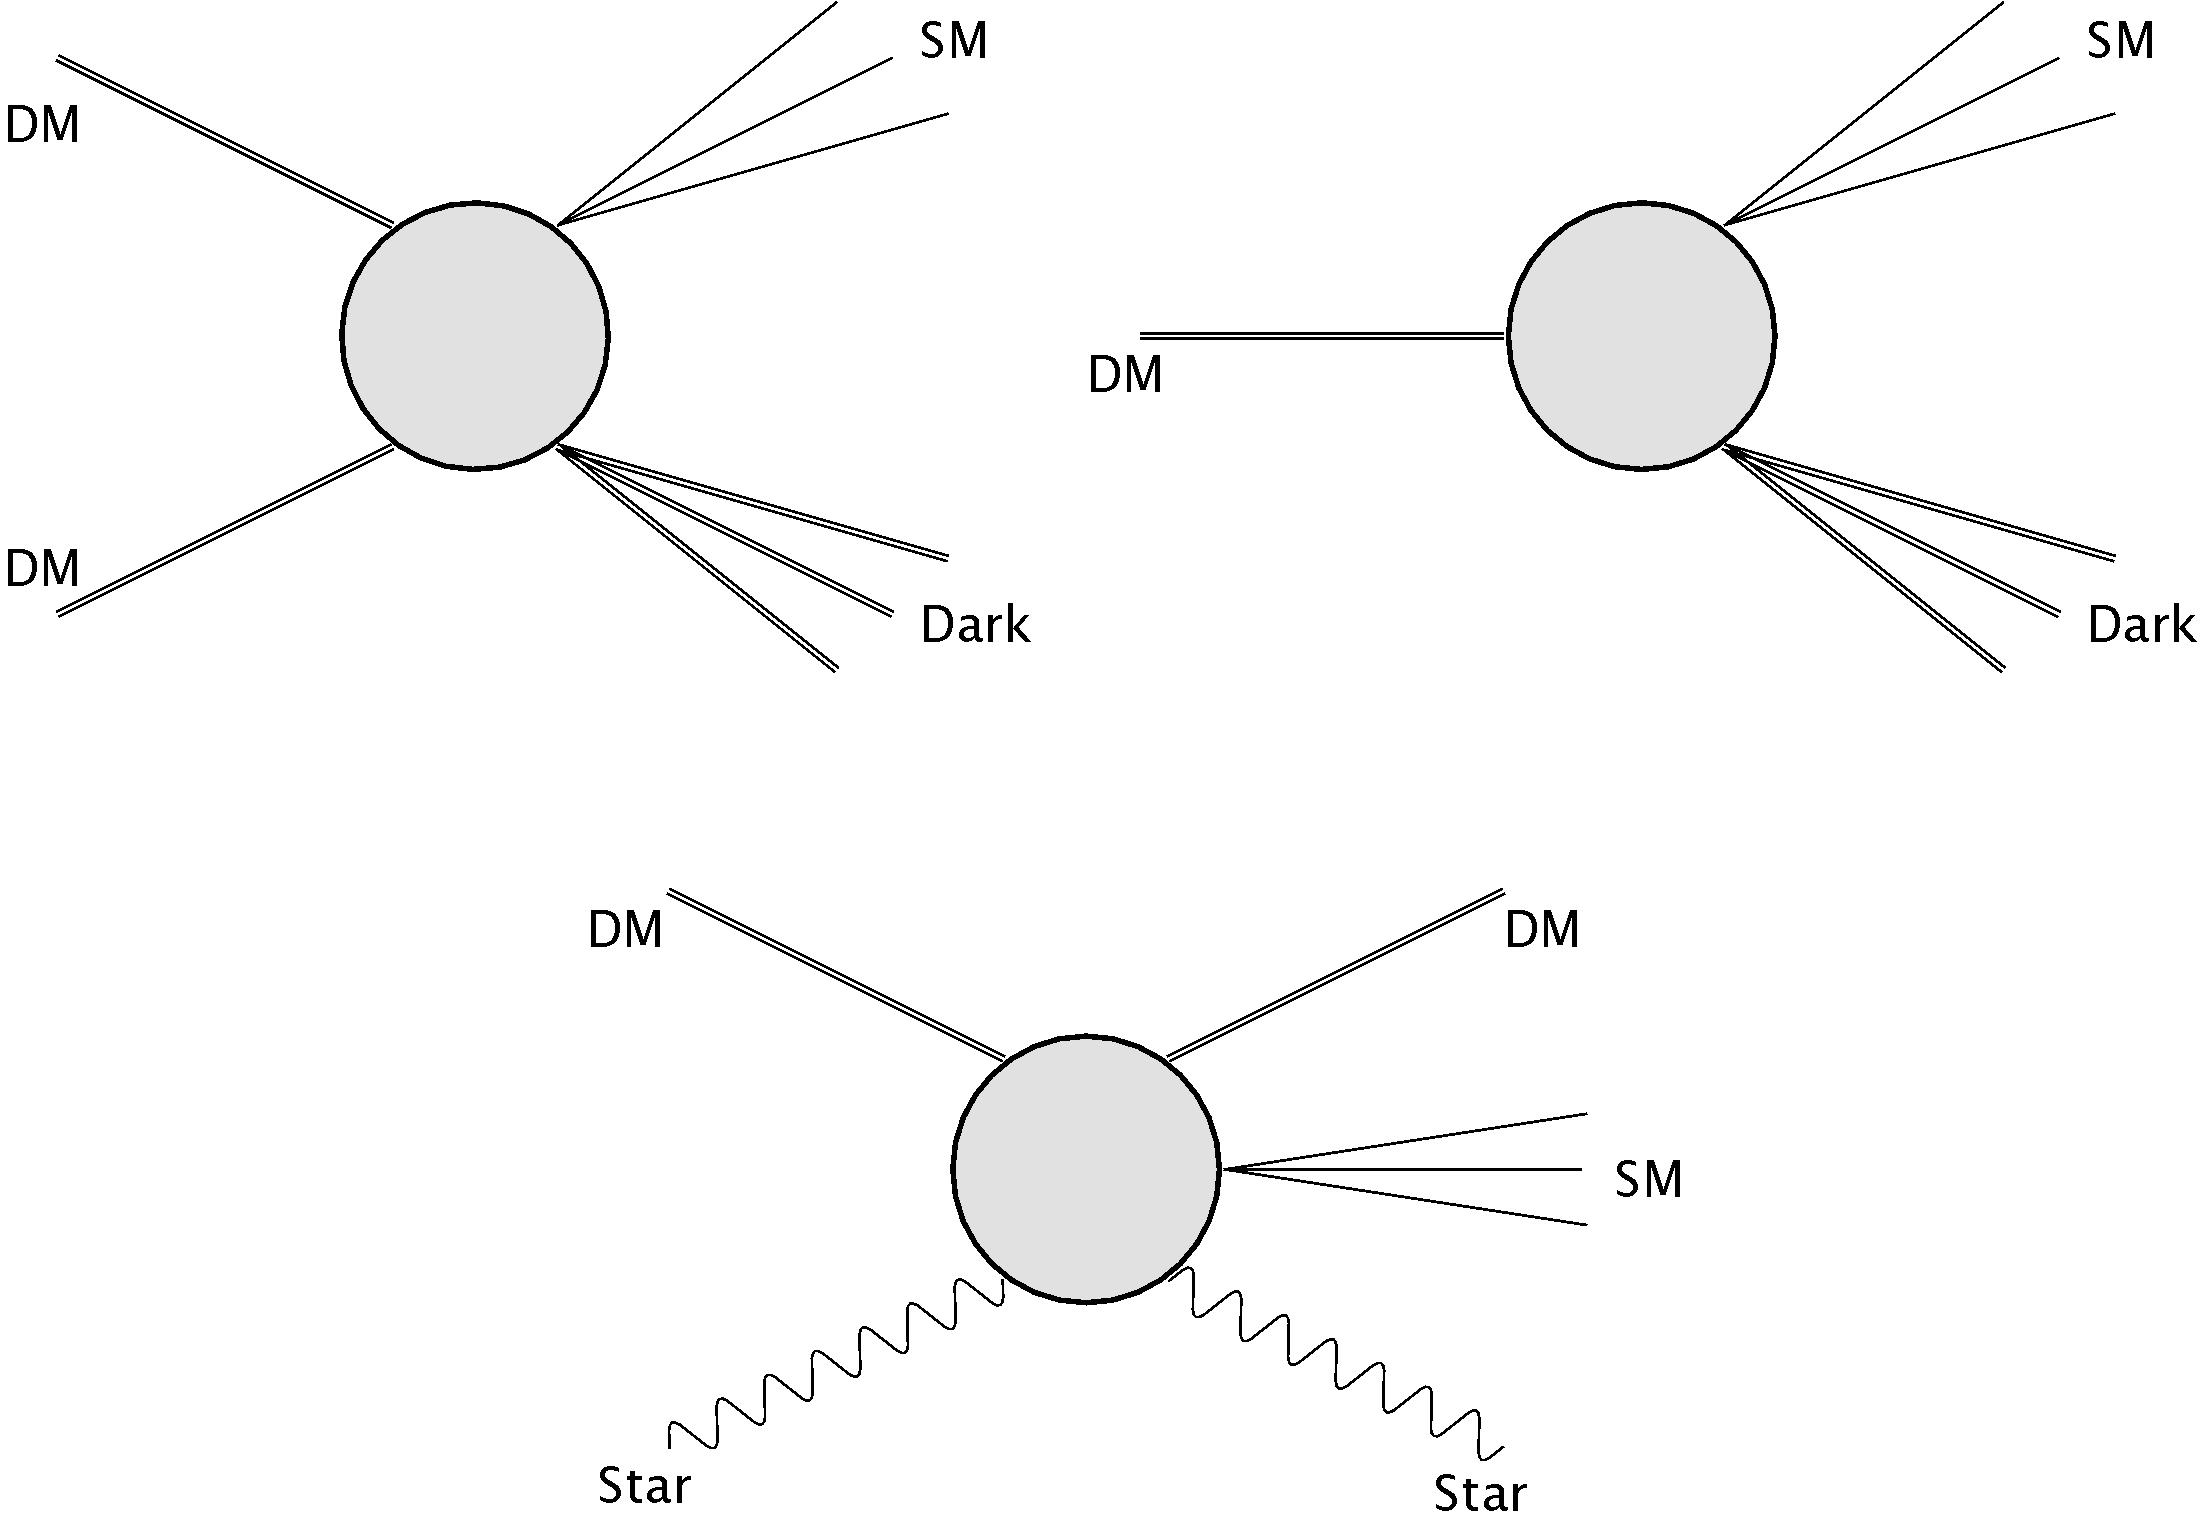
\includegraphics[scale=0.09]{feynmandiag.jpg}
\caption{Rough schematic of possible non-gravitational DM interactions in a WD. Heating of the WD occurs via the SM products, though also depicted are potential dark sector products.}
\label{fig:feynman}
\end{figure}

\subsection{Non-degenerate Shielding}
Runaway fusion only occurs in the degenerate WD interior where thermal expansion is suppressed as a cooling mechanism.
The outer layers of the WD, however, are composed of a non-degenerate gas and it is therefore essential that a DM candidate penetrate this layer in order to induce a SN. 
We parameterize this with a stopping power $(dE/dx)_\text{SP}$, giving the kinetic energy lost by the DM per distance traveled in the non-degenerate layer, and demand that 
\begin{align}
\label{eq:CrustCondition}
  \left( \frac{d E}{d x} \right)_\text{SP} \ll
  \frac{m_\text{DM} v^2_\text{esc}}{R_\text{crust}},
\end{align}
where $R_\text{crust} \sim 50 ~\text{km}$ is the width of a WD crust \cite{Chandrasekhar} and $v_\text{esc} \sim 10^{-2}$ is the escape velocity of a WD. \textcolor{blue}{double check these numbers}. 

\subsection{Transits}

\paragraph{Explosion Condition.}
The energy deposited in a continuous heating event is best described in terms of a linear energy transfer $(dE/dx)_\text{LET}$, which is the kinetic energy of SM particles produced per distance traveled by the DM.
If these products have a heating length $L_0$, then then relevant energy deposit as used in the general explosion condition \eqref{eq:energy_boom_condition} must be taken at minimum to be the energy transfered over the length $L_0$. 
We can always choose to consider the energy deposition over a longer segment of the DM trajectory, however by condition \eqref{eq:energy_boom_condition} such a deposition is \emph{less} explosive unless the length scale is smaller than the trigger size.
Thus, if $L_0 < \lambda_T$ we consider the deposition over the length $\lambda_T$, and otherwise over the larger scale $L_0$. 
We can take the energy of the DM to be roughly constant over this heating event, as for an explosive event any energy loss is subject to the condition 
\eqref{eq:CrustCondition} in order to penetrate the non-degenerate layer, which also guarantees negligible energy loss over the trigger size or heating lengths $L_0$.   
This yields the explosion condition for transit heating
\begin{align}
\label{eq:transitexplosion}
  \left( \frac{d E}{d x} \right)_\text{LET} \gtrsim 
  \frac{\Eboom}{\lambda_T} \cdot \text{Max} 
  \left[\frac{L_0}{\lambda_T}, 1 \right]^2.
\end{align}

The above argument sums the energy deposited along the DM trajectory as though it is all deposited simultaneously. 
This is only valid if the DM moves sufficiently quickly, so that the deposited energy does not diffuse out of the region of interest before the DM has traversed the region. 
We therefore require that the diffusion time $\tau_d$ across a heated region at temperature $T_f$ be larger than the DM crossing time:
\begin{align}
  \tau_d \sim \frac{L^2}{\alpha(T_f)} \gg 
  \frac{L}{v_\text{esc}},
\label{eq:SlowDiffusion}
\end{align}
where $\alpha(T)$ is the temperature-dependent diffusivity and DM transits at the stellar escape speed $v_\text{esc}$.
This condition is more stringent for smaller regions, so we focus on the smallest region of interest: $L = \lambda_T$. 
The condition \eqref{eq:SlowDiffusion} is then equivalent to demanding that the escape speed is greater than the conductive speed of the fusion wave front, $v_\text{cond} \sim \alpha(T_f) / \lambda_T$.
Values of $v_\text{cond}$ have been tabulated in \cite{Woosley}, and indeed condition \eqref{eq:SlowDiffusion} is satisfied for all WD densities.

\paragraph{SN Rate: Wind Scenario.}
The rate of transit events is given by the flux of DM passing through a WD
\begin{align}
  \Gamma_\text{transit} \sim 
  \frac{\rho_{\text{DM}}}{m_\text{DM}} R_\text{WD}^2 
  \l\frac{v_\text{esc}}{v}\r v_\text{esc}.
\label{eq:TransitFluxCondition}
\end{align} 
which contains an $\OO(100)$ enhancement due to gravitational focusing.

\section{Dark Matter Constraints}
\label{sec:Constraints}

We now constrain models of DM which will ignite a WD via one of the processes parameterized in Section \ref{sec:DMexplode}.
In order to do so, we will additionally assume a simple, schematic form for the DM interaction such that the heating length of the encounter can be calculated explicitly.
However, we first review the different ways in which white dwarfs can constrain DM candidates capable of triggering SN.

\subsection{Collisions and Decays}

\paragraph{Explosion Condition.}
For a point-like decay or collision event releasing particles of heating length $L_0$, ignition will occur if the total energy in SM products satisfies condition~\eqref{eq:energy_boom_condition}.
Such an event will likely result in both SM and dark sector products, so we parameterize the resulting SM energy as a fraction $f_\text{SM}$ of the DM mass.
Since we have non-relativistic, ultra-heavy DM, the DM mass is the dominant source of energy and therefore $f_\text{SM} \lesssim 1$ regardless of the interaction details, however we may well suspect that $f_\text{SM} \ll 1$ for realistic models.
With this parameterization, the explosion condition is
\begin{equation}
\label{eq:coldecay}
  m_\text{DM} f_\text{SM}  \gtrsim \Eboom \cdot \text{max} \left \{\frac{L_0}{\lambda_T}, 1 \right \}^3.
\end{equation}
We are thus sensitive to these events with for DM masses $m_\text{DM} \gtrsim 10^{16} ~\GeV$.

\paragraph{Event Rate: Wind Scenario.}
DM of mass $m_\text{DM}$ with negligible energy loss to the WD medium will traverse the star in roughly a time $R_\text{WD}/v_\text{esc}$ and have a number density within the WD of
\begin{equation}
n_\text{DM} \sim \frac{\rho_{\text{DM}}}{m_\text{DM}} \l \frac{v_\text{esc}}{v}\r,
\end{equation}
which includes an $\OO(10)$ gravitational enhancement to the DM number density.
Here $v_\text{esc} \sim 10^{-2} $ is the stellar escape velocity, $v \sim 10^{-3}$ the galactic virial velocity, and $\rho_\text{DM}$ the local energy density of DM.
The expected DM-DM collision rate parameterized by a cross-section $\sigma_\text{DM-DM}$ and net DM decay rate parameterized by a lifetime $\tau_\text{DM}$ are straightforward in the wind scenario,
\begin{align}
  \Gamma_\text{collision}
  &\sim n_\text{DM} \sigma_\text{DM-DM} v_\text{esc}
  \cdot n_\text{DM} R_\text{WD}^3 \\
  &\sim \l \frac{\rho_\text{DM}}{m_\text{DM}} \r^2 \sigma_\text{DM-DM} \l \frac{v_\text{esc}}{v}\r^2 v_\text{esc} R_\text{WD}^3 \\
  \label{eq:collisionDM}
  \Gamma_\text{decay}
  &\sim \frac{1}{\tau_\text{DM}} \cdot n_\text{DM} R_\text{WD}^3 \\
  &\sim \frac{1}{\tau_\text{DM}} \frac{\rho_{\text{DM}}}{m_\text{DM}} \l \frac{v_\text{esc}}{v}\r R_\text{WD}^3.
  \label{eq:taugamma}
\end{align}
If the DM interaction is explosive, these rates give the rate of DM-induced SN.

\paragraph{SN Rate: Capture Scenario.}
\textcolor{blue}{should probably add a citation somewhere here or above to Bru Monte}
We first review the evolution of DM within the star during a capture scenario.
As the DM rapidly loses energy it will thermalize with the star and slow to velocity
\begin{equation}
v_\text{th} \sim \sqrt{\frac{T}{m_\text{DM}}} \approx 10^{-12} \l \frac{10^{16} ~\GeV}{m_\text{DM}}\r^{1/2}
\end{equation}
where $T \sim \keV$ is the WD temperature.
It will then accumulate at the virial radius set by $v_\text{th}$
\begin{align}
  R_\text{vr} &\sim \l \frac{T}{G m_\text{DM} \rho_\text{WD}}\r^{1/2} \\
  &\approx 10^{-1} ~\text{cm} \l \frac{10^{16} ~\GeV}{m_\text{DM}}\r^{1/2}
  \l \frac{10^{31} ~\cm^{-3}}{n_\text{ion}}\r^{1/2}, \nonumber
\end{align}
where we have assumed the WD has roughly constant density within $R_\text{vr}$.
DM will collect at this radius until its total mass exceeds that of the WD medium within $R_\text{vr}$.
The DM cloud will then begin gravitational collapse.
The exact nature of this collapse is model-dependent, eventually being arrested by DM-DM interactions or the formation of a black hole.
In the case of composite DM, it is reasonable to suspect that the DM stabilizes into an inert core at a radius $R_\text{sta}$ larger than the Schwarzschild radius
\begin{align}
  R_\text{sch} \approx 10^{-24}~\text{cm}
  \l \frac{10^{16} ~\GeV}{m_\text{DM}}\r^{3/2}
  \l \frac{10^{31} ~\cm^{-3}}{n_\text{ion}}\r^{1/2}.
\end{align}
\textcolor{blue}{check these numbers}

There are several timescales relevant to this process.
The longest one is simply the time required for thermalized DM to drift down to the central core
\begin{align}
\label{eq:tdrift}
  t_\text{drift} &\sim R_\text{WD}/v_\text{th} \\
  &\approx 50 ~\text{yr} ~ \l \frac{m_\text{DM}}{10^{16} ~\GeV} \r^{1/2}.
\end{align}
This is much larger than the time need to collect a critical mass of DM, governed by the rate $\Gamma_\text{transit}$ of DM passing through the star
\begin{align}
\label{eq:tcol}
  t_\text{collect}
  &\sim \frac{\rho_\text{WD} R_\text{vr}^3}
  {m_\text{DM} \Gamma_\text{transit}} \\
  &\approx 10 ~\text{s} \l \frac{10^{16} ~\GeV}{m_\text{DM}} \r^{3/2}
  \l \frac{10^{31} ~\cm^{-3}}{n_\text{ion}}\r^{1/2}
\end{align}
or the timescale of the collapse itself
\begin{align}
  t_\text{collapse} &\sim R_\text{vr}/v_\text{th} \\
  &\approx 3 ~\text{s} ~ \l \frac{10^{31} ~\cm^{-3}}{n_\text{ion}}\r^{1/2}.
\end{align}
The core thus forms in a time $t_\text{drift}$, provided the mass of DM is sufficiently small - for masses $m_\text{DM} \gtrsim 10^{30}~\GeV$ the core will not form within the lifetime of the star.

For decay heating, capture gives an enhancement due to the increased number of DM particles within the WD.
This can be very large if the DM core admits decays, however it is still significantly enhanced over the wind scenario even for inert cores, as in the case that the DM forms a black hole.
In that case we have an enhancement of the net decay rate \eqref{eq:taugamma} by a factor
\begin{align}
  \frac{v_\text{esc}}{v_\text{th}}
  \approx 10^{10} \l \frac{m_\text{DM}}{10^{16}~\GeV} \r^{1/2}
\end{align}
due to the increased time spent by the DM in the WD medium before joining the inert core.

For DM-DM collision heating, it is possible that the collapse of the core will induce an ignition event due to the enhancement of DM number density during the collapse.
This would cap the lifetime of WDs to $t_\text{collect}$.
For a DM-DM collision cross-section $\sigma_\text{DM-DM}$, the collapse is explosive if
\begin{align}
  \frac{N^2 \sigma_\text{DM-DM}}{R_\text{sta}^2} \lesssim 1,
\end{align}
where $N$ is the total number of DM particles in the core,
\begin{align}
    N &\sim \frac{R^3_\text{vr} \rho_\text{WD}}{m_\text{DM}} \\
    &\approx 10^{21} \l \frac{10^{16} ~\GeV}{m_\text{DM}}\r^{5/2}
  \l \frac{10^{31} ~\cm^{-3}}{n_\text{ion}}\r^{1/2}. \nonumber
\end{align}
This will hold regardless of if the DM is collapsing in free fall or if the DM remains thermalized with the WD medium.
If the collapse itself is not explosive, there is still an enhanced SN rate relative to the wind scenario due to DM colliding while infalling to the core. Again we look at the conservative situation of an inert core - the rate is obviously much enhanced if the core is stabilized in a fluid state which admits DM-DM collisions.
The rate of infalling collisions is enhanced over the wind collision rate \eqref{eq:collisionDM} by a factor
\begin{align}
  \frac{v_\text{esc}}{v_\text{th}} \frac{R_\text{WD}}{R_\text{sta}}
  \approx 10^{20} \l \frac{m_\text{DM}}{10^{16}~\GeV} \r^{1/2}
  \l \frac{10^{-1}~\text{cm}}{R_\text{sta}} \r
\end{align}
<<<<<<< HEAD
which is an obnoxious $\approx 10^{40}$ enchantment for the case of collapse to a central black hole.

\subsection{Transits}

\paragraph{Explosion Condition.}
The energy deposited in a continuous heating event is best described in terms of a linear energy transfer $(dE/dx)_\text{LET}$, which is the kinetic energy of SM particles produced per distance traveled by the DM.
If these products have a heating length $L_0$, then then relevant energy deposit as used in the general explosion condition \eqref{eq:energy_boom_condition} must be taken at minimum to be the energy transfered over the length $L_0$. 
We can always choose to consider the energy deposition over a longer segment of the DM trajectory, however by condition \eqref{eq:energy_boom_condition} such a deposition is \emph{less} explosive unless the length scale is smaller than the trigger size.
Thus, if $L_0 < \lambda_T$ we consider the deposition over the length $\lambda_T$, and otherwise over the larger scale $L_0$. 
We can take the energy of the DM to be roughly constant over this heating event, as for an explosive event any energy loss is subject to the condition 
\eqref{eq:CrustCondition} in order to penetrate the non-degenerate layer, which also guarantees negligible energy loss over the trigger size or heating lengths $L_0$.   
This yields the explosion condition for transit heating
\begin{align}
\label{eq:transitexplosion}
  \left( \frac{d E}{d x} \right)_\text{LET} \gtrsim 
  \frac{\Eboom}{\lambda_T} \cdot \text{Max} 
  \left\{\frac{L_0}{\lambda_T}, 1 \right\}^2.
\end{align}

The above argument sums the energy deposited along the DM trajectory as though it is all deposited simultaneously. 
This is only valid if the DM moves sufficiently quickly, so that the deposited energy does not diffuse out of the region of interest before the DM has traversed the region. 
We therefore require that the diffusion time $\tau_d$ across a heated region at temperature $T_f$ be larger than the DM crossing time:
\begin{align}
  \tau_d \sim \frac{L^2}{\alpha(T_f)} \gg 
  \frac{L}{v_\text{esc}},
\label{eq:SlowDiffusion}
\end{align}
where $\alpha(T)$ is the temperature-dependent diffusivity and DM transits at the stellar escape speed $v_\text{esc}$.
This condition is more stringent for smaller regions, so we focus on the smallest region of interest: $L = \lambda_T$. 
The condition \eqref{eq:SlowDiffusion} is then equivalent to demanding that the escape speed is greater than the conductive speed of the fusion wave front, $v_\text{cond} \sim \alpha(T_f) / \lambda_T$.
Values of $v_\text{cond}$ have been tabulated in \cite{Woosley}, and indeed condition \eqref{eq:SlowDiffusion} is satisfied for all WD densities.

\paragraph{SN Rate: Wind Scenario.}
The rate of transit events is given by the flux of DM passing through a WD
\begin{align}
  \Gamma_\text{transit} \sim 
  \frac{\rho_{\text{DM}}}{m_\text{DM}} R_\text{WD}^2 
  \l\frac{v_\text{esc}}{v}\r v_\text{esc}.
\label{eq:TransitFluxCondition}
\end{align} 
which contains an $\OO(100)$ enhancement due to gravitational focusing.

\section{Dark Matter Constraints}
\label{sec:Constraints}

We now constrain models of DM which will ignite a WD via one of the processes parameterized in Section \ref{sec:DMexplode}.
In order to do so, we will additionally assume a simple, schematic form for the DM interaction such that the heating length of the encounter can be calculated explicitly.
However, we first review the different ways in which white dwarfs can constrain DM candidates capable of triggering SN.
=======
which is an obnoxious $\approx 10^{40}$ enhancement for the case of collapse to a central black hole.
>>>>>>> origin/master

\subsection{Review of WD Observables}
Following the discussion of \cite{Graham:2015apa}, our constraints come from (1)~the existence of heavy, long-lived white dwarfs, or (2)~the measured type Ia SN rate.
The typical age of a WD is of order the age of the universe $\sim \text{Gyr}$.
RX~J0648.04418 is a nearby star and one of the heaviest known WDs with a mass $\sim 1.25 ~M_{\odot}$ \cite{Mereghetti:2013nba}.
Of course, this is not the only known heavy WD - the Sloan Digital Sky Survey \cite{SDSS} has found $\sim 20$ others.
The NuStar collaboration has also recently uncovered evidence for the likely existence of $\sim 1.25 ~M_{\odot}$ WDs in the galactic center as well \cite{NuStar}.
Such candidates are particularly suited for our constraints as the energy deposit necessary to trigger SN $\Eboom$ is a decreasing function of WD mass.
However, less dense white dwarfs are significantly more abundant in the galaxy.
Thus, even if a sufficiently massive DM is unable to trigger a violent heating event within the lifetime of a WD, it could still ignite enough lighter WDs to affect the measured SN rate of $\sim $ 0.3 per century.
The DM-induced SN rate is estimated using the expected number of white dwarfs per galaxy $\sim 10^{10}$ and their mass distribution \cite{SDSS}.
Simulations indicate that only WD masses heavier than $\sim 0.85 ~M_{\odot}$ will result in optically visible SN \cite{Graham:2015apa}.
Therefore, most of the stars exploded in this manner will be in the mass range $\sim 0.85 - 1 ~M_{\odot}$, resulting in weaker SN than expected of typical Chandrasekhar mass WDs.

To summarize, a bound on DM parameters can be placed if either a single explosive event occurs during the lifetime of an observed star such as RX~J0648.04418, or the SN rate due to such DM events throughout the galaxy exceeds the measured value.
Note that for low-mass WDs dominated by photon diffusion, $\Eboom$ is a strong function of WD density.
In \cite{Graham:2015apa} the central WD density is used to constrain black hole transits with the justification that the density is nearly constant for much of the star.
The average density for WDs is typically a factor $\sim 10^{-2} - 10^{-1}$ less than the central density, although it is found that the WD density changes by an $\OO(1)$ fraction from the central value out at a distance $\sim R_\text{WD}/2$ \cite{Chandrasekhar}.
Therefore the central density is a valid approximation as long as we consider heating events within this ``modified" WD volume.
For simplicity, we employ this approach.


\subsection{Collision and Decay Constraints}
\label{sec:CollisionConstraints}

\paragraph{Schematic Constants}
We take $\rho_\text{DM} \sim 0.4 ~\GeV/\text{cm}^3$ for nearby stars, while for the white dwarfs observed in the galactic center it is estimated that $\rho_\text{DM} \sim 10^3 ~\text{GeV}/\text{cm}^3$ \cite{Nesti:2013uwa}.

We are able to constrain DM parameters whenever such processes are explosive according to the condition $\eqref{eq:coldecay}$.
Consider a schematic interaction where an annihilation or decay releases a number of SM particles $N_i$ of single species $i$ and individual energy $\epsilon$.
If we assume a fractional parameter $f_\text{SM}=1$, this corresponds to the entire mass of DM being converted into SM products $i$, each with energy $m_\text{DM}/N_i$.
These will deposit their energy and thermalize ions within a distance explicitly calculated in Section \ref{sec:SMHeating}.
The only caveat is that the computed interactions of SM particles extrapolated to energies beyond the Planck scale must be done with caution as gravitational effects may become important.
As a result, to adequately place constraints on ultra-heavy DM above this scale one can simply restrict the interactions to annihilations/decays into $N_i \gg 1$ particles of energy $\epsilon < 10^{18} ~\GeV$.


\paragraph{Complementary Limits}
It is important to note that there are additional limits on DM interactions of this kind, complementary to the limits placed from WDs.
For instance, DM can annihilate or decay into ultra-high energy particles within our galactic halo and therefore contribute to the cosmic ray flux seen in terrestrial air shower detectors.
As cosmic rays of energy greater than $\sim 10^{12} ~\GeV$ have not yet been observed \cite{ThePierreAuger:2015rha, AbuZayyad:2012ru}, this places a concrete limit on the DM interaction parameters $\sigma_\text{DM-DM}$ and $\tau_\text{DM}$ when such ultra-high energy particles are released.
In theory, a constraint may also be placed on lower-energy SM products from DM annihilations or decays which would provide an additional source for the measured cosmic ray flux, although such a detailed analysis is beyond the scope of this work.
The expected cosmic ray flux due to a DM decay in the galactic halo is given by:
\begin{equation}
\Gamma_\text{earth} \sim \int_{\text{halo}} \frac{\rho_\text{DM}(r)}{m_\text{DM}} \frac{R_\text{det}^2}{L^2} \frac{1}{\tau_\text{DM}},
\end{equation}
where $R_\text{det}^2 \sim (100 ~\text{km})^2$ denotes the typical surface area of a terrestrial cosmic ray detector and $L$ is the distance from the DM decay event to the earth.
$\rho_\text{DM}$ is the expected density profile of DM throughout the galactic halo.
This integral can be calculated numerically using an NFW profile fit (as given by \cite{Nesti:2013uwa}) and the known distance from the earth to the center of the galaxy, although to a very good approximation the result is the same if we simply set the galactic parameters to the average values $\rho_\text{DM} \sim 0.4 ~\GeV/\cm^3$ and $L \sim R_\text{halo} \sim 10 ~\text{kpc}$.
The constraint on DM is derived by requiring that the expected time for an event to strike earth $\Gamma_\text{earth}^{-1}$ is less than the lifetime of the detector $\sim 10 ~\text{yr}$.
Curiously, we find that in the case of DM decays the resulting bounds are of the same magnitude as those due to the observation of a local WD.
\textcolor{blue}{This coincidence can be seen explicitly by comparing the effective ``space-time volume" for the two detectors.
A cosmic ray detector sees events within a space-time volume $\sim (R_\text{det}^2 R_\text{halo} \times 10 ~\text{yr})$ which is numerically similar to the WD space-time volume for decay events $\sim (R_\text{WD}^3 \times 10 \times 10^9 ~\text{yr}$), where the additional $\OO(10)$ factor is due to the gravitational Sommerfeld enhancement.
Note that a similar calculation can be done in the case of DM-DM annihilations in the galactic halo, although in this case the gravitational enhancement is $\OO(10^3)$ and results in more stringent constraints from the WD observation.}
In addition, there are various cosmological bounds on DM interactions.
By requiring that the galactic halo has not diminished by more than an $\OO(1)$ factor during its lifetime, we can constrain $\sigma_\text{DM-DM}/m_\text{DM} \lesssim \text{barn}/\GeV$, valid regardless of the precise details of the collision.
The cosmological bound on DM lifetime $\tau_\text{DM} \gtrsim 100 ~\text{Gyr}$ is also independent of the nature of the decay products (see \cite{Poulin:2016nat} for details).
Note that a similar bound on DM self-interactions $\sigma_\text{DM-DM}/m_\text{DM}$ due to colliding clusters of galaxies \cite{Randall:2007ph} is of the same order of magnitude as that derived considering the depletion of own galaxy.
Since the limits imposed by the WD scale as $\sigma_\text{DM-DM} \propto m_\text{DM}^2$ and $\tau_\text{DM} \propto m_\text{DM}^{-1}$, there will necessary be a sufficiently large DM mass for which the above cosmological considerations are the more stringent constraints on its interactions.
Lastly, we briefly comment on the possibility for DM-DM collisions to affect the epoch of recombination and the observed properties of the cosmic microwave background (CMB).
This effect was first computed in \cite{Padmanabhan:2005es} to constrain DM annihilations into products that inject energy to the photon-baryon plasma and ionize neutral hydrogen and is of the form $\langle \sigma_\text{DM-DM} v \rangle \propto m_\text{DM}$.
Therefore, this could potentially be scaled to ultra-heavy DM masses if the cosmological history of such DM candidates is understood.

With the above schematic for DM-DM collisions, we place bounds on the cross section $\sigma_\text{DM-DM}$ as a function of $m_\text{DM}$ using the different classes of observation available and for representative choices of $f_\text{SM}$ and SM species $i$ released.
This is done in Figures \ref{fig:collisionclasses}, \ref{fig:collisioneta}, and \ref{fig:collisionspecies}.
In a similar manner, we constrain the lifetime $\tau_\text{DM}$ as a function of $m_\text{DM}$ in Figures \ref{fig:decayclasses}, \ref{fig:decayepsilon}, and \ref{fig:decayspecies}.


\begin{figure}
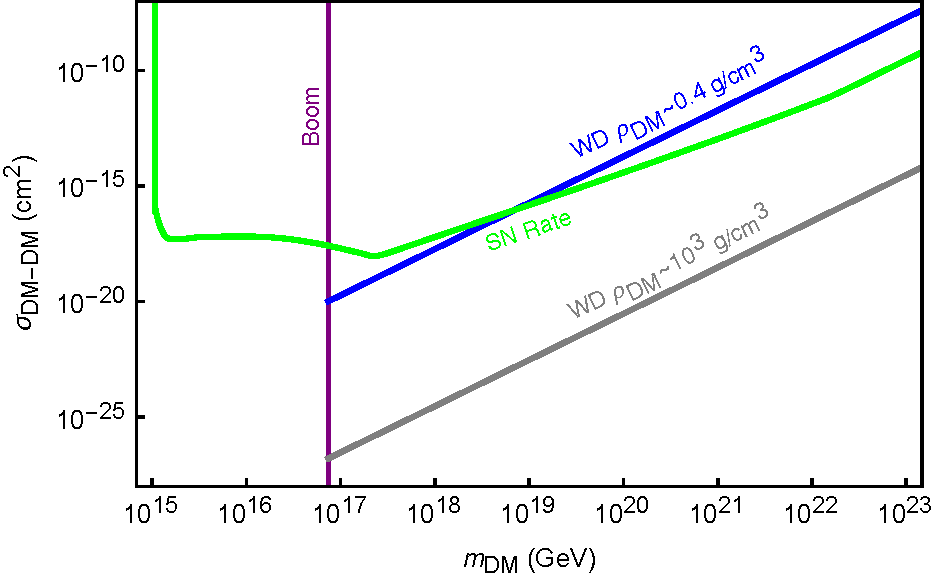
\includegraphics[scale=.45]{collisionobservation.pdf}
\caption{Constraints on DM-DM collision cross-section into photons with $f_\text{SM} =1$. Bounds come from observations of a single WD (local and galactic center) and measured SN rate}
\label{fig:collisionclasses}
\end{figure}

\begin{figure}
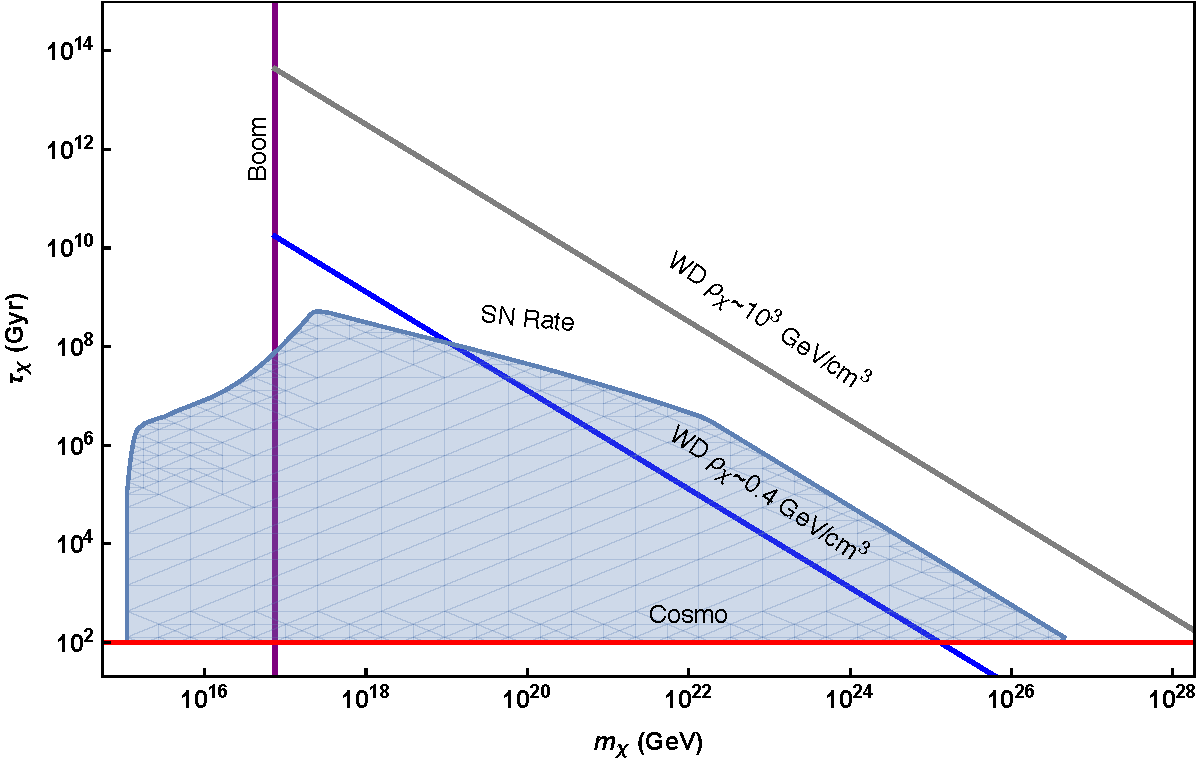
\includegraphics[scale=.45]{decayobservation.pdf}
\caption{Constraints on DM decay lifetime into photons with $f_\text{SM} =1$. Bounds come from observations of a single WD (local and galactic center) and measured SN rate}
\label{fig:decayclasses}
\end{figure}

\subsection{Transit Constraints}
\label{sec:TransitConstraints}

In order to constrain a DM model through its transit interaction with a WD, we require that it satisfy the explosive condition \eqref{eq:transitexplosion}.
This is given in terms of an LET, which parameterizes the ability for DM to release sufficient energy to the star in the form of SM particles.
$(dE/dx)_\text{LET}$ for any realistic DM model would necessarily involve a sum over stellar targets along with species that could be produced, as well as an integral over the produced particle spectrum.
However, consider a simplified interaction in which $\sigma_{i,\epsilon}$ denotes the cross-section for DM to scatter off a stellar constituent, producing a particle of species $i$ and and energy $\epsilon$.
If this were the only available channel for the DM to deposit energy, then the LET could be written as
\begin{align}
\label{eq:schematicLET}
  \left( \frac{d E}{d x} \right)_\text{LET} = n_\text{ion} \sigma_{i,\epsilon} \epsilon,
\end{align}
where we now specify to the case of DM collisions with nuclear targets.
Assuming such a DM-SM scattering interaction, the transit heating length is computed in Section~\ref{sec:SMHeating}.

In addition, we also make a sensible assumption that the LET $(dE/dx)_\text{LET}$ and DM stopping power $(dE/dx)_\text{SP}$ are equal for fixed number density - that is, the DM loses kinetic energy at the same rate as energy is deposited to the WD.
While such a statement is certainly not true for all DM models (such as the Q-ball, which liberates binding energy rather than transferring kinetic energy), it provides a useful benchmark to express constraints.
With this assumption, it is interesting to note that combining the transit explosion condition \eqref{eq:transitexplosion} with $\eqref{eq:schematicLET}$ yields a lower bound on DM mass such that the DM is able to both penetrate the crust \emph{and} trigger an explosion:
\begin{align}
\label{eq:transitmass}
m_\text{DM} > \Eboom \l \frac{R_\text{crust}}{\lambda_T} \r \l \frac{\rho_\text{crust}}{\rho_\text{central}} \r v_\text{esc}^2.
\end{align}
For the typical parameters of a $1.25 ~M_{\odot}$ WD we find that the DM mass must be greater than $\sim 10^{29} ~\GeV$ to ensure a bullet-like and explosive transit, taking the density of the WD crust $\rho_\text{crust}$ to be a nominal $\OO(10^{-2})$ fraction of the central density $\rho_\text{central}$.
In other words, if \eqref{eq:transitmass} were violated then the DM interaction is either not strong enough to ignite the WD or is so strong that the DM cannot penetrate the crust without losing appreciable kinetic energy.
However, it is important to note that this bound is only applicable when the energy input to the WD is chiefly coming from the DM kinetic energy, rather than binding energy or other sources.
With the above schematic for a DM transit, we constrain the parameter $\sigma_{i,\epsilon}$ as a function of DM mass $m_\text{DM}$.
This is done in Figures \ref{fig:transitclasses}, \ref{fig:transitepsilon}, and \ref{fig:transitspecies} using the different classes of observation available and for representative choices of $\epsilon$ and SM species $i$ released.

\begin{figure}
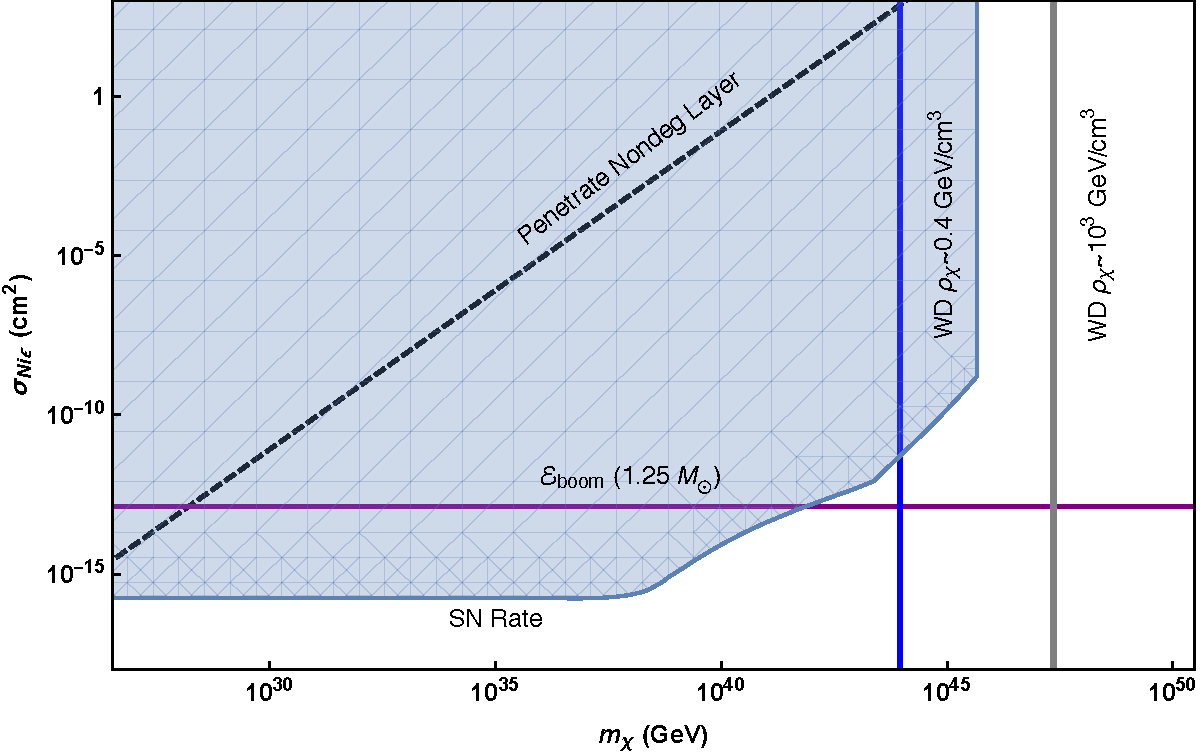
\includegraphics[scale=.45]{transitobservation.pdf}
\caption{Constraints on DM-nuclei scattering cross-section to produce photons of energy $\epsilon = \text{TeV}$. Bounds come from observations of a single WD (local and galactic center) and measured SN rate}
\label{fig:transitclasses}
\end{figure}

\section{Q-balls}
\label{sec:QBalls}

Having derived generic constraints on models of ultra-heavy DM in Section~\ref{sec:Constraints}, we turn towards a more concrete example: Q-balls.
In various supersymmetric extensions of the SM, non-topological solitons called Q-balls can be produced in the early universe \cite{Coleman:1985ki, Kusenko:1997si}.
If these Q-balls were stable, they would comprise a component of the DM today.
For gauge-mediated models with flat scalar potentials, the Q-ball mass and radius are given by
\begin{equation}
\label{eq:Qballprop}
M_Q \sim m_S Q^{3/4}, ~~~ R_Q \sim m_S^{-1} Q^{1/4},
\end{equation}
where $m_S$ is related to the scale of supersymmetry breaking, and $Q$ is the global charge of the Q-ball---in our case, baryon number.
The condition $M_Q/Q < m_p$ ensures that the Q-ball is stable against decay to nucleons.
When an (electrically neutral) baryonic Q-ball interacts with a nucleon, it absorbs its baryonic charge and induces the dissociation of the nucleon into free quarks.
During this proton decay-like process, $\sim \text{GeV}$ of energy is released through the emission of 2--3 pions.
We assume that for each Q-ball collision, there is equal probability to produce $\pi^0$ and $\pi^\pm$ under the constraint of charge conservation.

Note that a sufficiently massive Q-ball will become a black hole if the Q-ball radius is less than the Schwarzschild radius $R_Q \lesssim G M_Q$.
In the model described above, this translates into a condition $(M_\text{pl}/m_S)^4 \lesssim Q$.
For Q-ball masses of this order, gravitational interactions become relevant, though we will not consider those details here.
% Indeed, gravitational heating as in \cite{Graham:2015apa} may become more appropriate than the SM heating considered in this work.

We now determine the explosiveness of a Q-ball transit.
As in Section \ref{sec:Constraints}, this process is described by the parameter
\begin{equation}
\label{eq:QballLET}
\l\frac{dE}{dx}\r_\text{LET} \sim n_\text{ion} \sigma_Q N \epsilon,
\end{equation}
where the nuclear collision results in $N \sim 30$ pions released, each with kinetic energy $\epsilon \sim 500 ~\text{MeV}$.
These pions induce hadronic showers which terminate in low-energy hadrons that rapidly transfer their energy to ions via elastic scatters, as discussed in Section~\ref{sec:SMHeating}.
As a result, nearby ions heated over a region of size $L_0 \approx 10^{-6} ~\text{cm}$ \textcolor{red}{why not $10^{-7}$?} at a number density $n_\text{ion} \sim 10^{32}~\text{cm}^{-3}$.
$L_0$ scales inversely with $n_\text{ion}$ and is less than $\lambda_T$ for all WD densities.

Therefore, the Q-ball cross-section necessary to trigger runaway fusion is given by equations~\eqref{eq:transitexplosion} and~\eqref{eq:QballLET} to be
\begin{equation}
\sigma_Q \gtrsim \frac{1}{n_\text{ion}} \frac{\Eboom}{\lambda_T} \l \frac{T_f}{N \epsilon} \r.
\end{equation}
We see $\sigma_Q \approx 10^{-12} ~\text{cm}^2$ is sufficient to blow up a $\sim 1.25 ~M_{\odot}$ WD.
The cross-section for this interaction is approximately geometric
\begin{align}
\sigma_Q \sim \pi R_Q^2,
\end{align}
and thus we find that $Q \gtrsim 10^{42} ~(m_S/\text{TeV})^4$ can be adequately constrained from the observation of a single, heavy WD.
Note that the Q-ball-nuclear interaction described above results in minimal slowing or transfer of kinetic energy for Q-balls this massive, and as such condition \eqref{eq:CrustCondition} will be easily satisfied.

The strongest previous constraints on Q-balls come from Super-Kamiokande as well as air fluorescence detectors of cosmic rays \cite{Dine:2003ax}.
However, the constraints possible with the WD detector are in a fundamentally inaccessible region of parameter space for these terrestrial-based experiments due to the extremely low flux, and thus our new constraints are wholly complementary.
The strongest proposed limits due to the existence of a heavy WD in the galactic center are plotted in Figure~\ref{fig:Qballconstraint}. As a comparison, the combined limits from Super-K and the OA, TA cosmic ray detectors are shown in red.
\begin{figure}
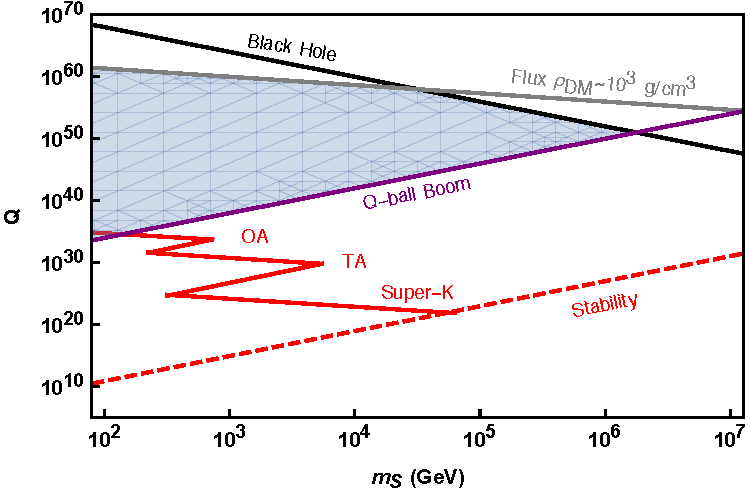
\includegraphics[scale=.55]{Qballconstraint.pdf}
\caption{Constraints on baryonic Q-balls from transits of a $\sim 1.25 ~M_{\odot}$ WD in the galactic center, $\rho_\text{DM} \sim 10^3 ~\text{g}/\text{cm}^3$. Also shown are the limits from Super-K and the OA, TA cosmic ray detectors, extracted from \cite{Dine:2003ax}.}
\label{fig:Qballconstraint}
\end{figure}

\section{Discussion}
\label{sec:Discussion}

It is clear that the detection of ultra-heavy DM is an open problem which will likely require a confluence of astrophysical probes.
Here we present a comprehensive guide to how white dwarfs can constrain such DM candidates that annihilate in, decay in, or transit through a WD and release sufficient energy to trigger a type Ia supernova.
In particular, we calculate the energy loss of high-energy particles due to SM interactions within the WD medium and determine the conditions for which a general energy deposition will heat a localized WD region to the critical size and temperature necessary for thermonuclear runaway.
The formalism provided will enable WDs to be applied as detectors for any DM models capable of heating the star through non-gravitational interactions, and as a concrete example we are able to place bounds on supersymmetric Q-ball DM over a wide region of parameter space.

In general, the phenomenology of such a DM-induced event will be the ignition of sub-Chandrasekhar mass progenitors.
This raises the tantalizing possibility that DM encounters with a WD can act as an alternative explosion mechanism and progenitor system for type Ia SN.
For decades, the standard lore has been that type Ia SN were due to the thermonuclear explosion of accreting carbon-oxygen white dwarfs in a binary system that reached the critical $\sim 1.4 ~M_{\odot}$ Chandrasekhar mass limit.
Since the Chandrasekhar mass is a value determined only by fundamental physics, it is natural to expect that the properties of type Ia SN are independent of initial conditions, enabling their use as ideal standard candles for precision luminosity distance measurements.
Nevertheless, it is well-known that such a mechanism cannot account for all observed type Ia SN.
In fact, recent observations \cite{Scalzo:2014sap, Scalzo:2014wxa} suggest that an $\OO(1)$ fraction of the observed type Ia SN appear to have sub-Chandrasekhar progenitors.
The leading explanation for this phenomenon is the detonation of a surface layer of helium which drives a shock into the interior of a sub-Chandrasekhar-mass WD \cite{Woosley1994,Fink:2007fv}.
However, in light of the lack of understanding of DM and its interactions, it is worthwhile to consider whether a DM-WD encounter may play the role of type Ia SN progenitor.

\begin{appendices}

\section{Particle Stopping in a White Dwarf}
\label{sec:Appendix}
Here we provide a detailed analysis of the electromagnetic and strong interactions in a carbon-oxygen WD, aimed towards calculating the energy loss per distance traveled of SM particles at an $\text{MeV}$ or greater.
We consider incident electrons, photons, pions, and nucleons.
The WD medium is very dense, with electron and ion number densities in the range $n_e = Z n_\text{ion} \sim 10^{31} - 10^{33} ~\cm^{-3}$ assuming $Z=6$.
Such high densities give rise to qualitatively different stopping behavior than is seen in terrestrial detectors.
Famously, the star is supported against collapse by electron degeneracy pressure.
For the WD masses we consider, the electrons are relativistic with a Fermi energy
\begin{equation}
  E_F \sim (3 \pi^2 n_e)^{1/3} \sim 1 -10 ~\MeV,
\end{equation}
which is significantly larger then the WD thermal temperature $T \sim \keV$ \textcolor{blue}{CITATION}.
The nuclei are a fully ionized, non-degenerate gas at the thermal temperature.
The strength of the Coulomb interaction energy relative to the temperature is described by the plasma parameter
\begin{equation}
\label{eq:lattice}
 \Gamma \sim \frac{Z^2 \alpha}{n_\text{ion}^{-1/3}T} \gg 1,
\end{equation}
indicating the ions are crystallized into a Coulomb lattice.
The ion plasma frequency is given by
\begin{align}
\Omega_p = \l \frac{4 \pi n_\text{ion} Z^2 \alpha}{m_\text{ion}}\r^{1/2} \sim 1 - 10~\text{keV},
\end{align}
where $m_\text{ion}$ is the ion mass.
As we will see, the thermal photons in the star never play a dominant role in stopping as the number density of photons $n_\gamma \sim T^3$ is orders of magnitude less than that of electrons and ions.

% \begin{figure}
% 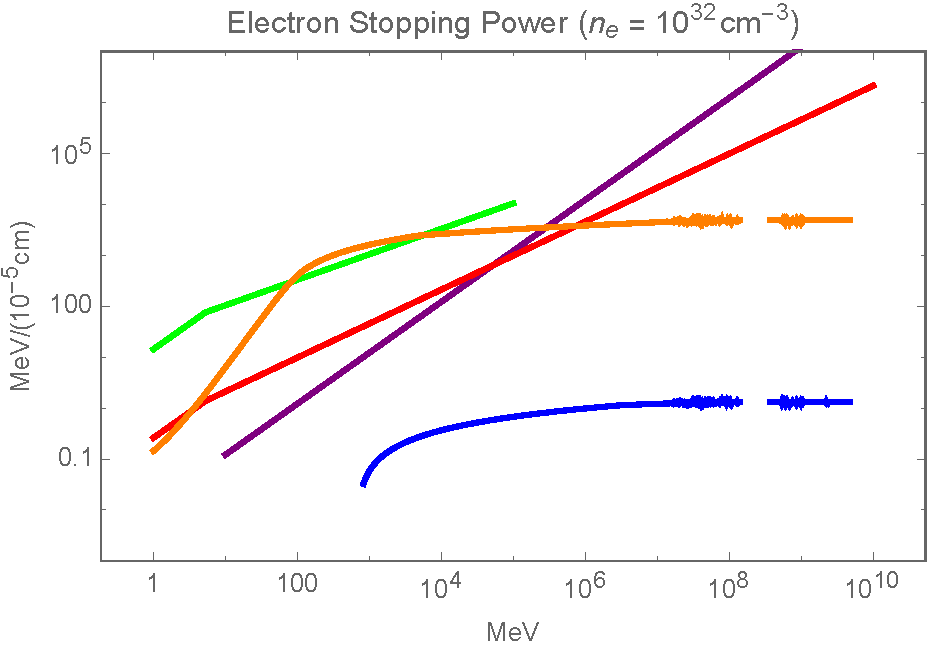
\includegraphics[scale=.60]{SPelectron.pdf}
% \caption{Electron energy loss in a WD density $n_e = 10^{33} ~\text{cm}^{-3}$}
% \label{fig:SPelectron}
% \end{figure}

% \begin{figure}
% 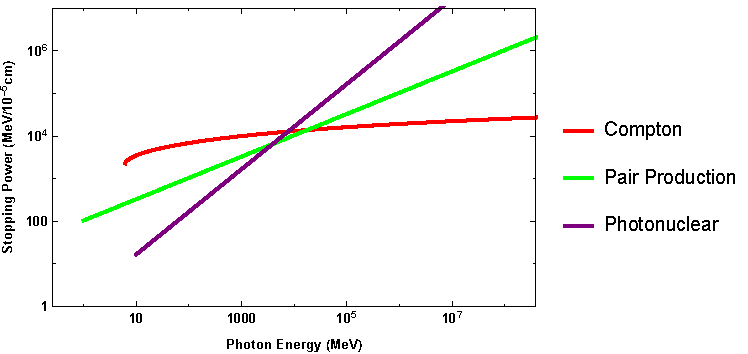
\includegraphics[scale=.60]{SPphoton.pdf}
% \caption{Photon energy loss in a WD density $n_e = 10^{33} ~\text{cm}^{-3}$}
% \label{fig:SPphoton}
% \end{figure}

% \begin{figure}
% 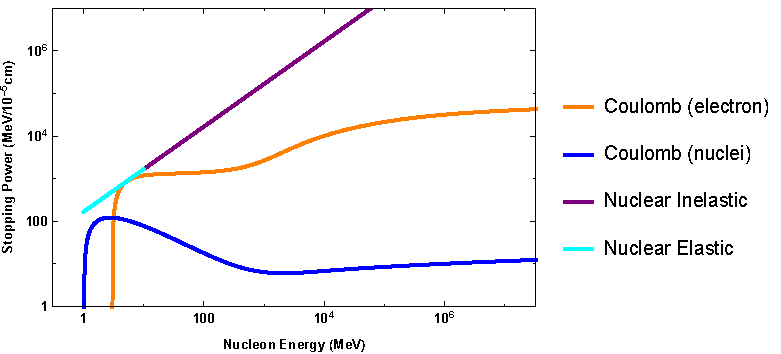
\includegraphics[scale=.60]{SPnucleon.pdf}
% \caption{Nucleon energy loss in a WD with density $n_e = 10^{33} ~\text{cm}^{-3}$. The Coulomb stopping powers apply only to protons.}
% \label{fig:SPnuc}
% \end{figure}

% \begin{figure}
% 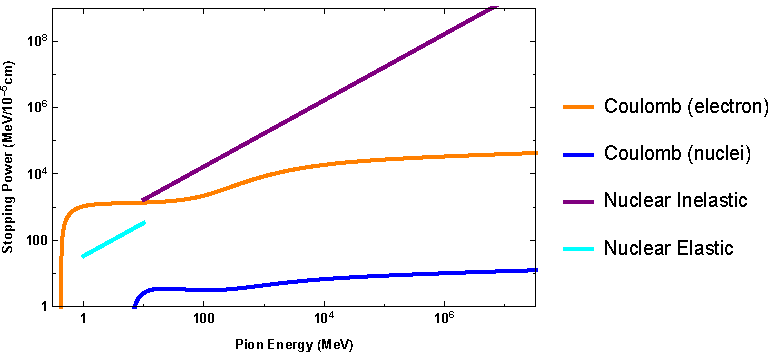
\includegraphics[scale=.60]{SPpion.pdf}
% \caption{Pion energy loss in a WD with density $n_e = 10^{33} ~\text{cm}^{-3}$. The Coulomb stopping powers apply only to charged pion.}
% \label{fig:SPpion}
% \end{figure}

\subsection{Coulomb Collisions off Ions}
The stopping power for Coulomb collisions with ions is most easily understood if we describe these scatters in terms of an impact parameter $b$.
Taking the ions to be at rest, consider an incident particle of mass $m$, charge $e$, and speed $\beta$ which transfers an energy $\omega$.
For soft scatters,
\begin{align}
  \label{eq:omega_soft}
  \omega \approx \frac{\alpha^2 Z^2}{2 m_\text{ion} \beta^2 b^2}
\end{align}
where $Z$ is the ion charge number and $m_\text{ion}$ the ion mass.
This is valid only for small $\omega$, and thus fails as $b\rightarrow0$.
While \eqref{eq:omega_soft} diverges for vanishing $b$, there is in fact a maximal energy transfer allowed by kinematics, $\omega_\text{kin}$.
For a stationary target $m_\text{ion}$, this occurs for an exactly backwards scatter and is given in full by
\begin{align}
  \omega_\text{kin} = \frac{2 m_\text{ion} p^2}{m_\text{ion}^2 + m^2 + 2E m_c}
\end{align}
where $p$, $E$ are the incoming momentum and energy, and the second expression is valid for large target masses.
For small $b$, the energy transfer will saturate at $\omega_\text{kin}$ and we can thus characterize the energy transfer as
\begin{align}
\label{eq:omega_piecewise}
    \omega \approx
    \begin{dcases}
    \;\;\;\; \omega_\text{kin}        & \, b < b_0 \\
    \frac{\alpha^2 Z^2}{2 m_\text{ion} \beta^2 b^2} & \, b > b_0
    \end{dcases}
\end{align}
where $b_0^2 = \alpha^2 Z^2 / 2 m_\text{ion} \beta^2 \omega_\text{kin}$ is a characteristic transition scale between hard and soft scatters.
The stopping power is given by integrating over all targets transverse to the incident particle's momentum
\begin{align}
\label{eq:stoppingpower_db}
    \frac{dE}{dx} =
        \int (n_\text{ion}\, d\sigma) \cdot \omega = n_\text{ion}
        \int \, 2\pi b \, db \cdot \omega.
\end{align}
This is a divergent quantity due to soft scatters ($b\rightarrow\infty$), corresponding to the infinite range of the Coulomb interaction.
In the WD medium, however, electron plasma screening cuts off soft scatters.
The screening length scale $\lambda_\text{tf}$ is given in the Thomas-Fermi approximation by \cite{Teukolsky}
\begin{align}
\label{eq:TF}
    \lambda_\text{tf}^{2} = \frac{E_F}{6 \pi \alpha n_e}
\end{align}
where $E_F$ is the electron Fermi energy.
The stopping power is
\begin{align}
  \frac{dE}{dx} &\approx n_\text{ion}
    \int_0^{\lambda_\text{tf}} \, 2\pi b  \, db \cdot \omega \\
    &\approx 2\pi n_\text{ion}\left(\omega_\text{kin}\int_0^{b_0} \, db \, b
    + \frac{\alpha^2 Z^2}{2 m_\text{ion} \beta^2}
    \int_{b_0}^{\lambda_\text{tf}} \,\frac{db}{b} \right)  \nonumber \\
    &= n_\text{ion} \frac{\pi \alpha^2 Z^2}{2 m_\text{ion} \beta^2}
      \, F\left(\frac{\lambda_\text{tf}}{b_0}\right)
      \label{eq:StoppingPowerOffIons}
\end{align}
where $F$ is a dimensionless factor
\begin{align}
    F(x) = \begin{dcases}
    x^2 & x < 1 \\
    1 + \log(x) & x > 1
  \end{dcases}
\end{align}
For low-energy, highly screened incident particles, $\lambda_\text{tf} < b_0$, this stopping power is simply $\sim \lambda_\text{tf}^2 \, \omega_\text{kin}$.
For high-energy particles, the screening enters only through the Coulomb logarithm.

Note that for incident electrons there is an additional upper bound on the energy transfer, $\omega_F = E - E_F$, as the electrons cannot be scattered into the Fermi sea.  If $\omega_F < \omega_\text{kin}$, then the above integrals should be taken with a lower limit of $b_F = \alpha^2 Z^2 / 2 m_\text{ion} \beta^2 \left(E - E_F\right)$ instead of zero.

One should also be careful about energy transfers smaller than the plasma frequency $\Omega_p \sim 1-10~\text{keV}$, for which phonon excitations may be important. A light incident particle with momentum $p$ and energy $E\ll m_\text{ion}$ would transfer momentum $q\lesssim p$ and energy $\omega_\text{free} = q^2/2 m_\text{ion}$ to a free ion. We therefore expect phonon effects to be important when $p^2/2 m_\text{ion} \lesssim \Omega_p$, and indeed one can check that the stopping power \eqref{eq:StoppingPowerOffIons} becomes dominated by energy transfers $\lesssim \Omega_p$ for this range of momenta. In this regime the ion is essentially a fixed target, and a simple Born approximation calculation yields a low-energy limit of the cross section $d \sigma$ used above in \eqref{eq:stoppingpower_db} and \eqref{eq:StoppingPowerOffIons}. For a free ion, arbitrarily small energy transfer $\omega$ is quantum mechanically permissible.

If we approximate the white dwarf as an Einstein solid instead, then each ion becomes a harmonic oscillator with frequency $\Omega_p$. The minimum permissible energy transfer is now $\omega = \Omega_p$, and we must compute the scattering cross section with the ion wave function in mind, transitioning from the harmonic oscillator ground state to the first excited state. This modifies the cross section by $|\bra{1}e^{i\textbf{q}\cdot \textbf{r}}\ket{0}|^2\approx q^2/2 m_\text{ion} \Omega_p$. (For similar cross section calculations, see \cite{Hofstadter}.) The stopping power integrand is therefore modified from
\begin{align}
(n_\text{ion}\, d\sigma)\cdot\omega_\text{free} \to (n_\text{ion}\, d\sigma\cdot\frac{q^2}{2 m_\text{ion}\Omega_p})\cdot \Omega_p
\end{align}
However, since $\omega_\text{free} = q^2/2 m_c$ at these energies, the two stopping powers are the same. Scatters are rarer at incident momenta $p^2/2 m_\text{ion} \lesssim \Omega_p$ where phonons matter, but each scatter transfers more energy so that the stopping power is equivalent.


\subsection{Coulomb Collisions off Electrons}

Coulomb scattering off degenerate electrons has two additional features compared to scattering off ions: the electron targets are not stationary, and they require a threshold energy transfer in order to be scattered out of the Fermi sea.
This qualitatively changes the behavior of the stopping power.
The combined effect of these features is not obvious, though it can be understood by straightforward heuristic arguments which we present below.
In addition, the full result can be calculated numerically.
The scattering rate between an incident particle and the population of electrons with a given momentum $\vec{q}$ can be found easily in the center-of-mass frame.
The stopping power then follows by boosting this result to the WD rest frame, calculating the corresponding energy transfers, and summing over the electron momentum distribution including only those scatters that excite electrons above the Fermi sea.
This calculation is well-approximated by the limiting cases described below, as shown in Figure~\textcolor{blue}{plot of coulomb-electron stopping powers}.

\subsubsection{Non-relativistic Incident Particles}
Consider first the limit of a slow incident particle of mass $m \gg m_e$, charge number $Z$, and incident momentum $\vec{p}$ with $m \gg p$.
This scatters off relativistic Fermi sea electrons.
As the electron speeds are much faster than the incident, a target electron with momentum $\vec{q}$ will scatter to leading order with only a change in direction,
\begin{align}
  \delta \vec{q} \approx q \left(\hat{q}_{out} - \hat{q}_{in}\right).
\end{align}
This results in an energy $\omega$ transfered from the incident,
\begin{align}
  \omega &\approx \frac{p^2}{2 m} -
    \frac{\left(\vec{p} - \delta \vec{q}\right)^2}{2 m} \\
    &\approx -\frac{q^2}{2m}  \left(\hat{q}_{out} - \hat{q}_{in}\right)^2
  + \frac{q p}{2m} \hat{p} \cdot \left(\hat{q}_{out} - \hat{q}_{in}\right).
\end{align}
If the incident momentum $p$ is smaller than the electron momentum $q$, the incident particle nominally gains energy from the electron.
This cannot happen, however, as there no phase space for an electron to lose energy within the Fermi sea.
We thus expect a cutoff in the stopping power for incident momenta near the Fermi momentum.
For all incident species except electrons this occurs at energies below our region of interest, and so we proceed with $q \lesssim p$:
\begin{align}
  \omega &\approx \frac{q p}{2m}
  \hat{p} \cdot \left(\hat{q}_{out} - \hat{q}_{in}\right).
\end{align}

Before computing the stopping power, consider the relative important of Pauli blocking and plasma screening.
Both of these effects achieve the same qualitative result, preventing the softest scatters from occurring.
The Pauli effect will suppress scatters with energy transfer less than roughly the Fermi energy, while plasma screening suppresses scatters at impact parameter above $\lambda_\text{tf}$.
This corresponds to a momentum transfer
\begin{align}
      \delta q_\text{tf} \approx \frac{\alpha Z}{\beta \lambda_\text{tf}}
\end{align}
and energy transfer
\begin{align}
  \label{eq:cuttoff_compare}
  \omega_\text{tf} \sim \frac{p}{2m} \frac{\alpha Z}{\beta \lambda_\text{tf}}
         \sim 5 \cdot 10^{-2} \frac{p}{m} E_f.
\end{align}
This is always going to be less than the Fermi energy for non-relativistic incident particles, and so we can ignore the plasma cutoff in favor of the Pauli cutoff.

At leading order the electron is not aware of the small ion velocity, so scattering occurs with the recoilless, relativistic Mott cross section
\begin{align}
    \frac{d\sigma}{d\hat{q}_{out}} \approx \frac{\alpha^2 Z^2}{4\pi q^2}
    \frac{\cos^2\left(\frac{\theta}{2}\right)}
    {\sin^4\left(\frac{\theta}{2}\right)}
\end{align}
where we have taken the electron speed to be nearly $1$ and $\cos\theta = \hat{q}_{out} \cdot \hat{q}_{in}$.
The incident particle will lose energy off relativistic electrons $\vec{q}$ at a rate
\begin{align}
  \frac{dE}{dt} &\approx dn \int d{\hat{q}_{out}}
    \frac{d\sigma}{d\hat{q}_{out}} \omega \cdot
    \Theta\left(\omega - q_f + q\right)
\end{align}
where $dn$ indicates the number density of electrons with momentum $\vec{q}$ and the Heavyside function enforces the Pauli energy threshold.
Now summing over all target electrons with the Fermi distribution
\begin{align}
  \frac{dn}{d^3q} = n_e \frac{3}{4\pi q_f^3} \, \Theta(q_f - q)
\end{align}
and noting that the stopping power is given by $v_\text{ion}^{-1} (dE/dt)$, we have the full stopping power
\begin{align}
  \frac{dE}{dx} \approx \; &n_e \frac{3 \alpha^2 Z^2}{32 \pi^2 q_f^3}
    \cdot \Bigg[ \\
  &\int_0^{q_f} dq \, q \, \Theta\left(\omega - q_f + q\right) \nonumber \\
  &\int d\hat{q}_{in} \, d\hat{q}_{out}
   \frac{\cos^2\left(\frac{\theta}{2}\right)}
        {\sin^4\left(\frac{\theta}{2}\right)}
   \, \hat{p} \cdot \left(\hat{q}_{out} - \hat{q}_{in}\right)
     \Bigg] \nonumber.
\end{align}
The integral over target electron momenta selects only those near the top of the Fermi sea,
% \begin{align}
%   \int &dq \, q \, \Theta\left(\omega - q_f + q\right) \Theta(q_f - q) \\
%   &\approx \int_0^{q_f} dq \, q \; \Theta\left[\frac{q p}{2m} \hat{p} \cdot
%   \left(\hat{q}_{out}-\hat{q}_{in}\right)-E_f+q\right] \\
%   &= \frac{1}{2} q_f^2 \left[ 1 - \frac{1}
%   {\left(1 + \frac{p}{2m}
%   \hat{p}\cdot\left(\hat{q}_{out}-\hat{q}_{in}\right)\right)^2} \right]   \\
%   &\approx \frac{1}{2} q_f^2 \frac{p}{m}
%   \hat{p}\cdot\left(\hat{q}_{out}-\hat{q}_{in} \right)
% \end{align}
simplifying this to
\begin{align}
  \frac{dE}{dx} &\approx \, n_e \frac{\alpha^2 Z^2}{E_f} \frac{p}{m} \, I_a
\end{align}
where $I_a \approx 10$ is a dimensionless angular integral that is independent of target or incident properties:
\begin{align}
   I_a &= \frac{3}{64\pi^2} \int d\hat{q}_{in} \, d\hat{q}_{out}
   \frac{\cos^2\left(\frac{\theta}{2}\right)}
        {\sin^4\left(\frac{\theta}{2}\right)}
   \, \left[\hat{p} \cdot \left(\hat{q}_{out} - \hat{q}_{in}\right)\right]^2
\end{align}

\subsubsection{Relativistic Incident Particles}

Now consider a fast incident particle of mass $m \gg m_e$, charge number $Z$, and incident momentum $\vec{p}$ with $m \ll p$.
The relative velocity between a target electron and the incident particle is of the same order as the ion's incident velocity itself, and we therefore expect the scattering to proceed, up to $\OO(1)$ factors, as though the electron were stationary.
We take the energy transfer $\omega$ to be given by Equation~\eqref{eq:omega_piecewise} with the target mass $m_\text{ion}$ replaced by the electron momentum $q$, which provides the appropriate target inertia in this context.
% \begin{align}
%     \omega \approx
%     \begin{dcases}
%     \; \omega_\text{kin}        & \, b < b_0 \\
%     \frac{\alpha^2 Z^2}{2 q b^2} & \, b > b_0
%     \end{dcases}
% \end{align}
The stopping is then given by the Pauli-blocked generalization of Equation~\eqref{eq:stoppingpower_db}
\begin{align}
\label{eq:stoppingpower_db}
  &\begin{aligned}  \frac{dE}{dx} = \Bigg[
      \int &dq \, n_e \frac{3}{4\pi q_f^3} \, \Theta(q_f - q) \, \cdot \\
      \int &db \, 2\pi b \, \omega \,
      \Theta\left(\omega - q_f + q\right) \Bigg]. \end{aligned} \\
  &\hphantom{\frac{dE}{dx}}
    \approx n_\text{e} \frac{2\pi \alpha^2 Z^2}{E_f}
    \, G\left(\frac{\omega_\text{kin}}{E_f}\right).
\end{align}
where the dimensionless factor $G$ is given by a Pauli integral
\begin{align}
    G\left(x\right) =
    \begin{dcases}
    \frac{1}{3} x^3 - \frac{3}{2} x^2 + 3 x & x < 1 \\
    \;\;\;\, \frac{11}{6} + \log\left(x\right) & x > 1. \\
    \end{dcases}
\end{align}
For large enough incident momenta, the plasma screening will provide the appropriate soft scatter cutoff instead of the Pauli cutoff used here.
This can be see by Equation~\eqref{eq:cuttoff_compare}.
However, in this regime the cutoff enters only through the Coulomb logarithm and so the difference is a matter of immaterial $\OO(1)$ factors.



\subsection{Compton and Inverse Compton Scattering}

Photons and charged particles can elastically exchange energy through Compton scattering.
We focus first on an incident photon losing energy to the WD medium.
Since the cross-section for this process scales inversely with the target mass, the stopping due to photon-ion collisions will be far subdominant to photon-electron collisions and we ignore the former.
Consider an incident photon of energy $k$ scattering off an electron of energy $\sim E_F$.
In the rest frame of the electron, this cross-section is given by the Klein-Nishina formula
\begin{equation}
\label{KN}
  \frac{d\sigma_\text{KN}}{d (\cos \theta)} = \frac{\pi \alpha^2}{m_e^2}
  \l \frac{k^\prime}{k} \r^2
  \l \frac{k^\prime}{k} + \frac{k}{k^\prime} -\sin^2 \theta \r
\end{equation}
where $k^\prime$ is the outgoing photon energy, related to the scattering angle $\theta$ by the Compton formula
\begin{equation}
{k^{\prime }={\frac {k}{1+{\frac {k}{m_e}}(1-\cos \theta )}}}.
\end{equation}
In the limit $k > m_e$, the cross-section is suppressed by the incoming energy $\sigma_\text{KN} \sim \frac{\alpha^2}{m_e k}$.
The outgoing photons will scatter predominately in a near-forward direction $\cos \theta \approx m_e/k$ so that $k^\prime \sim m_e$.
Thus the typical photon energy loss is large, and cooling proceeds via a small number of hard scatters.
The Compton stopping power is estimated to be
\begin{equation}
\label{eq:approx-comptonSP}
  - \l\frac{dk}{dx}\r \sim \frac{n_e \alpha^2}{m_e} \l 1 - \frac{m_e}{k} \r.
\end{equation}
A more detailed analysis computes the stopping power as
\begin{equation}
\label{eq:comptonSP}
  -\l\frac{dk}{dx}\r =  \int d (\cos \theta) n_e \frac{d\sigma_\text{KN}}{d (\cos \theta)} \l k - k^\prime \r,
\end{equation}
with an appropriate Lorentz boost to the electron rest frame, although the full result only differs from the above estimate by $\OO(1)$ factors.
Further, Pauli-blocking of the target electrons is taken into account using a modified number density as in \eqref{eq:pauliblocking}.
We find that degeneracy only introduces a significant suppression when $k \lesssim 10 ~\text{MeV}$, which is to be expected since the interaction is dominated by hard, near-forward scatters.

We now briefly consider incident electrons which may cool by inverse Compton scatters with the thermal bath of photons in the WD.
The number density of these photons is set by the temperature of the star $n_\gamma \sim T^3 \sim 10^{23} ~\cm^{-3}$, where we have taken $T \sim \text{keV}$.
As this is parametrically smaller than the number density of electrons, it is reasonable to suspect that the energy loss due to inverse Compton scattering is far subdominant to electron-electron collisions.
An estimate in the manner of \eqref{eq:approx-comptonSP} gives the inverse Compton stopping power in terms of the photon temperature $T$ and incident electron energy $E$
\begin{equation}
\label{eq:invcomptonSP}
  -\l \frac{dE}{dx}\r \sim
  \begin{cases}
    \alpha^2 \frac{T^4}{m_e^4} E^2 & E \lesssim \frac{m_e^2}{T} \\
    \alpha^2 T^2 & E \gtrsim \frac{m_e^2}{T} \\
  \end{cases},
\end{equation}
where the change in scaling with $E$ marks a transition from Thompson-like scattering in the electron rest frame to suppressed high-energy scattering.
As expected, we find that the inverse Compton stopping power is negligible compared to Coulomb scattering.

\subsection{Bremsstrahlung and Pair Production with LPM Suppression}

Bremsstrahlung and pair production can be a dominant stopping mechanisms for high-energy electrons and photons.
We restrict our attention to radiative processes off target nuclei rather than target electrons as the latter are additionally suppressed by degeneracy, kinematic recoil, and charge factors.
The cross-section for an electron of energy $E$ to radiate a photon of energy $k$ is given by the Bethe-Heitler formula
\begin{equation}
\label{eq:BH}
\frac{d \sigma_\text{BH}}{dk} = \frac{1}{3 k n_\text{ion} X_0} (y^2+2 [1+ (1-y)^2]), ~~~ y = k/E.
\end{equation}
$X_0$ is the radiation length, and is generally of the form
\begin{equation}
\label{eq:radiationlength}
X_0^{-1} = 4 n_\text{ion} Z^2 \frac{\alpha^3}{m_e^2} \log{\Lambda}, ~~~ \log{\Lambda} \sim \int \frac{1}{b}.
\end{equation}
where $\log{\Lambda}$ is a logarithmic form factor containing the maximum and minimum effective impact parameters allowed in the scatter.
Integrating \eqref{eq:BH}, we find the energy loss due to bremsstrahlung is simply
\begin{equation}
-\l\frac{dE}{dx}\r \sim \frac{E}{X_0}.
\end{equation}
In \eqref{eq:radiationlength}, the minimum impact parameter is set by a quantum-mechanical bound such that the radiated photon frequency is not larger than the initial electron energy.
For a bare nucleus, this distance is the electron Compton wavelength.
It is important to note that collisions at lesser impact parameters will still radiate but with suppressed intensity.
The maximum impact parameter is set by the distance at which the nuclear target is screened.
For an atomic target this is of order the Bohr radius, and for nuclear targets in the WD this is the Thomas-Fermi screening radius given by \eqref{eq:TF}.
%Evidently, there exists a critical electron number density $n_e \sim 10^{32} ~\text{cm}^{-3}$ for which the logarithmic form factor appears to vanish.
For our purposes, we simply take $\log{\Lambda} \sim \OO(1)$ for all WD densities under consideration and refrain from a full quantum-mechanical calculation at small impact parameters.

However, bremsstrahlung will be suppressed by the ``Landau-Pomeranchuk-Migdal" (LPM) effect - see \cite{Klein:1998du} for an extensive review.
High-energy radiative processes involve very small longitudinal momentum transfers to nuclear targets ($\propto k/E^2$ in the case of bremsstrahlung).
Quantum mechanically, this interaction is delocalized across a formation length over which amplitudes from different scattering centers will interfere.
This interference turns out to be destructive and must be taken into account in the case of high energies or high-density mediums.
Calculations of the LPM effect can be done semi-classically based on average multiple scattering.
It is found that bremsstrahlung is suppressed for $k < E(E-k)/E_\text{LPM}$, where
\begin{equation}
\label{eq:LPM}
E_\text{LPM} = \frac{m_e^2 X_0 \alpha}{4 \pi}.
\end{equation}
For the WD densities in which radiative energy loss is considered, $E_\text{LPM} \sim 1-10^{2} ~\text{MeV}$.
The degree of suppression is found to be
\begin{equation}
\frac{d\sigma_\text{LPM}/dk}{d\sigma_\text{BH}/dk} = \sqrt{\frac{k E_\text{LPM}}{E (E-k)}},
\end{equation}
so that the bremsstrahlung stopping power in the regime of high-suppression is modified
\begin{equation}
\label{eq:bremloss}
-\l\frac{dE}{dx}\r_\text{LPM} \sim \l\frac{E_\text{LPM}}{E} \r^{1/2} \frac{E}{X_0}, ~~~ E>E_\text{LPM}.
\end{equation}
We find that the LPM effect diminishes energy loss due to soft radiation so that the radiative stopping power is dominated by single, hard bremsstrahlung.

In addition to the LPM effect, other forms of interaction within a formation length will suppress bremsstrahlung when $k \ll E$.
The emitted photon can coherently scatter off electrons and ions in the media, acquiring an effective mass of order the plasma frequency $\omega_p$.
Semi-classically, this results in a suppression of order $(k/\gamma \omega_p)^2$ when the radiated photon energy $k < \gamma \omega_p$.
This is known as the ``dielectric effect".
For high-energy electrons, this dielectric suppression only introduces a minor correction to \eqref{eq:bremloss}, in which soft radiation is already suppressed by the LPM effect \cite{Klein:1998du}.

We now briefly summarize the stopping of photons via pair production. Similar to \eqref{eq:BH}, the cross-section for a photon of energy $k$ to produce an electron-positron pair with energies $E$ and $k-E$ is
\begin{equation}
\label{eq:PP}
\frac{d \sigma_\text{BH}}{dE} = \frac{1}{3 k n_\text{ion} X_0} (1+ 2[x^2+ (1-x)^2]) ~~~ x = E/k,
\end{equation}
valid beyond the threshold energy $k \gtrsim m_e$.
As a result, the pair production cross-section $\sim 1/(n_\text{ion} X_0)$.
However, the LPM effect suppresses pair production at energies $E(k-E) > k E_\text{LPM}$ so that the cross-section reduces to
\begin{equation}
\sigma_{pp} \sim \l\frac{E_\text{LPM}}{k} \r^{1/2} \frac{1}{n_\text{ion} X_0}, ~~~ E>E_\text{LPM}.
\end{equation}
Note that the LPM effect is less significant for higher-order electromagnetic processes since these generally involve larger momentum transfers for the same final-state kinematics.
Thus, when the suppression factor exceeds $\OO(\alpha)$, these interactions should also be considered.
For instance, the energy loss due to electron direct pair production $eN \to e^+ e^- e N$ has been calculated in \cite{Gerhardt:2010bj} and is found to exceed that of bremsstrahlung at an energy $\sim 10^{8} ~\GeV$.
A similar crossover is to be expected for other higher-order diagrams as well, although such a calculation is beyond the scope of this work.
Rather, at such high energies the stopping power is dominated by photonuclear and electronuclear interactions anyway, and we may simply ignore the contributions from other radiative processes \cite{Kleinconvo}.

\subsection{Nuclear Interactions}

Nuclear interactions can be either elastic or inelastic - the nature of the interaction is largely determined by the incident particle energy.
Elastic collisions are most significant for energy loss at scales less than the nuclear binding energy $\sim 10 ~\text{MeV}$.
A single, backward elastic scatter could result in an incident particle losing virtually all of its energy if the incident and target masses are the same.
However, we will be primarily concerned with light hadrons incident on relatively heavy nuclei, i.e. ping-pong balls bouncing around a sea of bowling balls.
An elastic collision between a incident, non-relativistic hadron of mass $m$, kinetic energy $E$ and a stationary nuclear target of mass $M$ results in an average final energy
\begin{equation}
\label{eq:elasticratio}
E' \sim \l \frac{m}{M}\r E, ~~~~ m < M,
\end{equation}
where it is assumed there is an isotropic distribution in the center-of-mass scattering angle.
Above $\sim \text{MeV}$, it is found that electrostatic repulsion is negligible for nuclear interactions of protons and $\pi^+$.
Therefore, the stopping power for any light hadron due to elastic collisions is of the form
\begin{equation}
- \l \frac{dE}{dx} \r \sim \l \frac{m}{M} \r \frac{E}{l_\text{el}}.
\end{equation}
$l_\text{el}$ denotes the mean free path for elastic collisions characterized by cross-section $\sigma_\text{el}$.
Above $10 ~\MeV$ the nuclear elastic cross-section approaches the geometric cross-section for carbon $\sim 100 ~\text{mb}$, while at $\MeV$ energies the elastic cross section generally rises to be of order $\sim \text{b}$.
At intermediate energies $1 - 10 ~\MeV$, the interaction is dominated by various nuclear resonances \cite{Tavernier}.
For our purposes, we will conservatively estimate the elastic cross section for nucleons and pions to be $\sigma_\text{el} \approx 1 ~\text{b}$ when $E \lesssim 10 ~\MeV$, and ignore the energy loss due to elastic scatters at higher energies where inelastic processes will dominate.

Now we determine the stopping power due to inelastic nuclear collisions at $E \gtrsim 10 ~\MeV$.
In such a collision, an incoming hadron interacts with one or more nucleons in the nucleus to produce a $\OO(1)$ number of additional hadrons which approximately split the initial energy.
For incident energies greater than the nucleon binding energy $\sim \GeV$, the majority of secondary hadrons are pions which carry transverse momentum of order $\sim 100 ~\MeV$ \cite{Tavernier}.
In addition, during this process the target nucleus is broken up.
The nuclear fragment is typically left in an unstable state with negligible center-of-mass recoil, and relaxes via the slow emission of low-energy $\sim \MeV$ hadrons and photons.
Note that for incident hadrons in the range $10 ~\MeV - \GeV$, it is found that roughly equal fractions of protons, neutrons, and pions are emitted after each inelastic collision \cite{Pionnuclear}.
In either case, if secondary hadrons are sufficiently energetic then they will induce further inelastic collisions.
A roughly collinear hadronic shower is the result of all such interactions caused by primary and secondary particles.
This cascade is adequately described by a radiative stopping power
\begin{equation}
\label{eq:nucshower}
-\l \frac{dE}{dx}\r \sim \frac{E}{l_\text{inel}},
\end{equation}
neglecting of $\OO(1)$ logarithmic factors.
$l_\text{inel}$ is the inelastic nuclear mean free path characterized by an inelastic cross-section $\sigma_\text{inel}$.
At these energies, $\sigma_\text{inel} \approx 100 ~\text{mb}$ and is roughly constant in energy.
The shower will end once final-state hadrons reach a critical energy - this is either the scale at which an additional mechanism dominates the stopping power or the nuclear binding energy $\sim 10 ~\MeV$.

Photons of energy $k \gtrsim 10 ~\text{MeV}$ can also strongly interact with nuclei through the production of virtual quark-antiquark pairs.
Photonuclear interactions are similar in nature to the inelastic collisions of hadrons, although the cross-section $\sigma_{\gamma A}$ is roughly a factor $\approx \alpha$ smaller.
Below $\sim \GeV$ the photonuclear cross-section is complicated by nuclear resonances while above $\sim \GeV$, $\sigma_{\gamma A}$ is a slowly increasing function of energy \cite{Tavernier}.
At sufficiently high energies, photonuclear interactions can in fact become coherent with the photon interaction spread over multiple nuclei \cite{Gerhardt:2010bj}.
This coherence will further reduce the photonuclear mean free path $l_{\gamma A}$.
As a conservative estimate, at energies $k \gtrsim 10 ~\text{MeV}$ we assume a constant photonuclear cross-section of order $\sigma_{\gamma A} \approx \text{mb}$.
Similarly, electrons can also lose energy by radiating a virtual photon that interacts hadronically with a nearby nucleus.
Naively we would expect the electronuclear stopping power to parametrically be of the form $(dE/dx) \sim E \alpha/l_{\gamma A}$.
A more detailed calculation in \cite{Gerhardt:2010bj} obtains a similar result but with an additional $\OO(10)$ numerical factor.
\end{appendices}

\section*{Acknowledgements}
We would like to thank Keisuke Harigaya, Spencer Klein, Jacob Leedom, Robert McGehee, and Lian-Tao Wang for stimulating discussions.

\begin{thebibliography}{99}
\bibliographystyle{unsrt}

%\cite{Akerib:2016vxi}
\bibitem{Akerib:2016vxi}
  D.~S.~Akerib {\it et al.} [LUX Collaboration],
  %``Results from a search for dark matter in the complete LUX exposure,''
  Phys.\ Rev.\ Lett.\  {\bf 118}, no. 2, 021303 (2017)
  doi:10.1103/PhysRevLett.118.021303
  [arXiv:1608.07648 [astro-ph.CO]].
  %%CITATION = doi:10.1103/PhysRevLett.118.021303;%%
  %431 citations counted in INSPIRE as of 03 Nov 2017

%\cite{Agnese:2017njq}
\bibitem{Agnese:2017njq}
  R.~Agnese {\it et al.} [SuperCDMS Collaboration],
  %``Results from the Super Cryogenic Dark Matter Search (SuperCDMS) experiment at Soudan,''
  arXiv:1708.08869 [hep-ex].
  %%CITATION = ARXIV:1708.08869;%%
  %3 citations counted in INSPIRE as of 03 Nov 2017

%\cite{Graham:2015apa}
\bibitem{Graham:2015apa}
  P.~W.~Graham, S.~Rajendran and J.~Varela,
  %``Dark Matter Triggers of Supernovae,''
  Phys.\ Rev.\ D {\bf 92}, no. 6, 063007 (2015)
  %doi:10.1103/PhysRevD.92.063007
  [arXiv:1505.04444 [hep-ph]].
  %%CITATION = doi:10.1103/PhysRevD.92.063007;%%
  %29 citations counted in INSPIRE as of 28 Sep 2017


\bibitem{Woosley}
 F.~X. Timmes and S.~E. Woosley, Astro. Phys. Journal {\bf 396}, 649 (1992).

%\cite{Gasques:2005ar}
\bibitem{Gasques:2005ar}
  L.~R.~Gasques, A.~V.~Afanasjev, E.~F.~Aguilera, M.~Beard, L.~C.~Chamon, P.~Ring, M.~Wiescher and D.~G.~Yakovlev,
  %``Nuclear fusion in dense matter: Reaction rate and carbon burning,''
  Phys.\ Rev.\ C {\bf 72}, 025806 (2005)
  %doi:10.1103/PhysRevC.72.025806
  [astro-ph/0506386].
  %%CITATION = doi:10.1103/PhysRevC.72.025806;%%
  %59 citations counted in INSPIRE as of 28 Sep 2017


\bibitem{cococubed}
F.~X.~Timmes, http://cococubed.asu.edu/code pages/coldwd.shtml

%\cite{Formaggio:2013kya}
\bibitem{Formaggio:2013kya}
  J.~A.~Formaggio and G.~P.~Zeller,
  %``From eV to EeV: Neutrino Cross Sections Across Energy Scales,''
  Rev.\ Mod.\ Phys.\  {\bf 84}, 1307 (2012)
  %doi:10.1103/RevModPhys.84.1307
  [arXiv:1305.7513 [hep-ex]].
  %%CITATION = doi:10.1103/RevModPhys.84.1307;%%
  %207 citations counted in INSPIRE as of 28 Sep 2017


\bibitem{Chandrasekhar}
S.~Chandrasekhar, ``An Introduction to the Study of Stellar Structure", University of Chicago press (1939).

%\cite{Mereghetti:2013nba}
\bibitem{Mereghetti:2013nba}
  S.~Mereghetti,
  %``RX J0648.0--4418: the fastest-spinning white dwarf,''
  %doi:10.1142/9789814623995_0469
  arXiv:1302.4634 [astro-ph.HE].
  %%CITATION = doi:10.1142/9789814623995_0469;%%
  %3 citations counted in INSPIRE as of 28 Sep 2017


\bibitem{SDSS}
S.~J.~Kleinman, S. O. Kepler, D. Koester, I. Pelisoli  {\it et al.}, Astrophys. J. Suppl. {\bf 204}, article
id. 5, 14 pp. (2013)

\bibitem{NuStar}
K.~Perez, C.~J.~Hailey, F.~E.~Bauer, {\it et al.}, Nature {\bf 520}, 646 (2015)

%\cite{Nesti:2013uwa}
\bibitem{Nesti:2013uwa}
  F.~Nesti and P.~Salucci,
  %``The Dark Matter halo of the  Milky Way, AD 2013,''
  JCAP {\bf 1307}, 016 (2013)
  %doi:10.1088/1475-7516/2013/07/016
  [arXiv:1304.5127 [astro-ph.GA]].
  %%CITATION = doi:10.1088/1475-7516/2013/07/016;%%
  %108 citations counted in INSPIRE as of 28 Sep 2017


%\cite{ThePierreAuger:2015rha}
\bibitem{ThePierreAuger:2015rha}
  A.~Aab {\it et al.} [Pierre Auger Collaboration],
  %``Measurement of the cosmic ray spectrum above 4 $\times$ 10$^{18}$ eV using inclined events detected with the Pierre Auger Observatory,''
  JCAP {\bf 1508}, 049 (2015)
  %doi:10.1088/1475-7516/2015/08/049
  [arXiv:1503.07786 [astro-ph.HE]].
  %%CITATION = doi:10.1088/1475-7516/2015/08/049;%%
  %22 citations counted in INSPIRE as of 28 Sep 2017


%\cite{AbuZayyad:2012ru}
\bibitem{AbuZayyad:2012ru}
  T.~Abu-Zayyad {\it et al.} [Telescope Array Collaboration],
  %``The Cosmic Ray Energy Spectrum Observed with the Surface Detector of the Telescope Array Experiment,''
  Astrophys.\ J.\  {\bf 768}, L1 (2013)
  %doi:10.1088/2041-8205/768/1/L1
  [arXiv:1205.5067 [astro-ph.HE]].
  %%CITATION = doi:10.1088/2041-8205/768/1/L1;%%
  %189 citations counted in INSPIRE as of 28 Sep 2017


%\cite{Poulin:2016nat}
\bibitem{Poulin:2016nat}
  V.~Poulin, P.~D.~Serpico and J.~Lesgourgues,
  %``A fresh look at linear cosmological constraints on a decaying dark matter component,''
  JCAP {\bf 1608}, no. 08, 036 (2016)
  %doi:10.1088/1475-7516/2016/08/036
  [arXiv:1606.02073 [astro-ph.CO]].
  %%CITATION = doi:10.1088/1475-7516/2016/08/036;%%
  %24 citations counted in INSPIRE as of 28 Sep 2017


%\cite{Randall:2007ph}
\bibitem{Randall:2007ph}
  S.~W.~Randall, M.~Markevitch, D.~Clowe, A.~H.~Gonzalez and M.~Bradac,
  %``Constraints on the Self-Interaction Cross-Section of Dark Matter from Numerical Simulations of the Merging Galaxy Cluster 1E 0657-56,''
  Astrophys.\ J.\  {\bf 679}, 1173 (2008)
  %doi:10.1086/587859
  [arXiv:0704.0261 [astro-ph]].
  %%CITATION = doi:10.1086/587859;%%
  %323 citations counted in INSPIRE as of 28 Sep 2017


%\cite{Padmanabhan:2005es}
\bibitem{Padmanabhan:2005es}
  N.~Padmanabhan and D.~P.~Finkbeiner,
  %``Detecting dark matter annihilation with CMB polarization: Signatures and experimental prospects,''
  Phys.\ Rev.\ D {\bf 72}, 023508 (2005)
  %doi:10.1103/PhysRevD.72.023508
  [astro-ph/0503486].
  %%CITATION = doi:10.1103/PhysRevD.72.023508;%%
  %186 citations counted in INSPIRE as of 28 Sep 2017


%\cite{Coleman:1985ki}
\bibitem{Coleman:1985ki}
  S.~R.~Coleman,
  %``Q Balls,''
  Nucl.\ Phys.\ B {\bf 262}, 263 (1985)
  Erratum: [Nucl.\ Phys.\ B {\bf 269}, 744 (1986)].
  %doi:10.1016/0550-3213(85)90286-X, 10.1016/0550-3213(86)90520-1
  %%CITATION = doi:10.1016/0550-3213(85)90286-X, 10.1016/0550-3213(86)90520-1;%%
  %676 citations counted in INSPIRE as of 28 Sep 2017


%\cite{Kusenko:1997si}
\bibitem{Kusenko:1997si}
  A.~Kusenko and M.~E.~Shaposhnikov,
  %``Supersymmetric Q balls as dark matter,''
  Phys.\ Lett.\ B {\bf 418}, 46 (1998)
  %doi:10.1016/S0370-2693(97)01375-0
  [hep-ph/9709492].
  %%CITATION = doi:10.1016/S0370-2693(97)01375-0;%%
  %450 citations counted in INSPIRE as of 28 Sep 2017


%\cite{Dine:2003ax}
\bibitem{Dine:2003ax}
  M.~Dine and A.~Kusenko,
  %``The Origin of the matter - antimatter asymmetry,''
  Rev.\ Mod.\ Phys.\  {\bf 76}, 1 (2003)
  %doi:10.1103/RevModPhys.76.1
  [hep-ph/0303065].
  %%CITATION = doi:10.1103/RevModPhys.76.1;%%
  %373 citations counted in INSPIRE as of 28 Sep 2017


%\cite{Scalzo:2014sap}
\bibitem{Scalzo:2014sap}
  R.~Scalzo {\it et al.} [Nearby Supernova Factory Collaboration],
  %``Type Ia supernova bolometric light curves and ejected mass estimates from the Nearby Supernova Factory,''
  Mon.\ Not.\ Roy.\ Astron.\ Soc.\  {\bf 440}, no. 2, 1498 (2014)
  %doi:10.1093/mnras/stu350
  [arXiv:1402.6842 [astro-ph.CO]].
  %%CITATION = doi:10.1093/mnras/stu350;%%
  %33 citations counted in INSPIRE as of 28 Sep 2017


%\cite{Scalzo:2014wxa}
\bibitem{Scalzo:2014wxa}
  R.~A.~Scalzo, A.~J.~Ruiter and S.~A.~Sim,
  %``The ejected mass distribution of type Ia supernovae: A significant rate of non-Chandrasekhar-mass progenitors,''
  Mon.\ Not.\ Roy.\ Astron.\ Soc.\  {\bf 445}, no. 3, 2535 (2014)
  %doi:10.1093/mnras/stu1808
  [arXiv:1408.6601 [astro-ph.HE]].
  %%CITATION = doi:10.1093/mnras/stu1808;%%
  %34 citations counted in INSPIRE as of 28 Sep 2017


 \bibitem{Woosley1994}
  %Sub--Chandrasekhar Mass Models for Type IA Supernovae
  S.~E.~Woosley and T.~A.~Weaver, Astrophysical Journal {\bf 423}, pp.371-379 (1994).

%\cite{Fink:2007fv}
\bibitem{Fink:2007fv}
  M.~Fink, W.~Hillebrandt and F.~K.~Roepke,
  %``Double-detonation supernovae of sub-Chandrasekhar mass white dwarfs,''
  Astron.\ Astrophys.\
  [Astron.\ Astrophys.\  {\bf 476}, 1133 (2007)]
  %doi:10.1051/0004-6361:20078438
  [arXiv:0710.5486 [astro-ph]].
  %%CITATION = doi:10.1051/0004-6361:20078438;%%
  %72 citations counted in INSPIRE as of 28 Sep 2017


\bibitem{Rossi}
B.~Rossi, ``High Energy Particles", Prentice-Hall, Inc., Englewood Cliffs, NJ (1952).

\bibitem{Jackson}
J.~D.~Jackson, ``Classical Electrodynamics", 3rd edition, John Wiley and Sons, New
York, (1998).

\bibitem{Teukolsky}
S.~L.~Shapiro and S.~A.~Teukolsky, ``Black Holes, White Dwarfs, and Neutron Stars", Wiley (1983).

%\cite{Klein:1998du}
\bibitem{Klein:1998du}
  S.~Klein,
  %``Suppression of Bremsstrahlung and pair production due to environmental factors,''
  Rev.\ Mod.\ Phys.\  {\bf 71}, 1501 (1999)
  %doi:10.1103/RevModPhys.71.1501
  [hep-ph/9802442].
  %%CITATION = doi:10.1103/RevModPhys.71.1501;%%
  %151 citations counted in INSPIRE as of 28 Sep 2017

%\cite{Gerhardt:2010bj}
\bibitem{Gerhardt:2010bj}
  L.~Gerhardt and S.~R.~Klein,
  %``Electron and Photon Interactions in the Regime of Strong LPM Suppression,''
  Phys.\ Rev.\ D {\bf 82}, 074017 (2010)
  %doi:10.1103/PhysRevD.82.074017
  [arXiv:1007.0039 [hep-ph]].
  %%CITATION = doi:10.1103/PhysRevD.82.074017;%%
  %24 citations counted in INSPIRE as of 28 Sep 2017

\bibitem{Kleinconvo}
S.~Klein, private communication

\bibitem{Tavernier}
S.~Tavernier, "Experimental Techniques in Nuclear and Particle Physics", Springer (2010).

\bibitem{Pionnuclear}
T.~S.~H.~Lee and R.~P.~Redwine,
 %``Pion-Nucleus Interactions",
 Annu. Rev. Nucl. Part. Sci {\bf 52}, pp.23-63 (2002)


\end{thebibliography}

\end{document}
